
In this chapter a search for highly ionizing, short tracks is presented. The chapter will be structured as follows:
In \mbox{Sec.~\ref{sec:Motivation}} a motivation will be given, followed by an overview of the general search strategy in \mbox{Sec.~\ref{sec:GeneralSearchStrategy}}.
As the variable \dedx plays a crucial role in this analysis, a general introduction and different possible parametrizations will be introduced in \mbox{Sec.~\ref{sec:DeDxMeasurement}}.
In this context also the conducted offline calibration of the silicon pixel detector will be explained.
After presenting the simulated SM and signal samples which were used in this analysis (\mbox{Sec.~\ref{sec:SimulatedSamples}}) the event selection is shown (Sec.~\ref{sec:EventSelection}).
Then, the various sources of background are charecterized (Sec.~\ref{sec:SourcesOfBackgrounds}) and the methods to estimate their size are presented (\ref{sec:BackgroundEstimation}).
As a final step an optimization in the search sensitivity was done, which can be found in Sec.~\ref{sec:Optimization}.
The chapter concludes by presenting the results of this analysis in Sec.~\ref{sec:Results}, and after a short introduction to the statistical methods of limit setting (Sec.~\ref{sec:LimitSetting}), the results will be interpreted in the context of Supersymmetry (Sec.~\ref{sec:Interpretation}).


%%%%%%%%%%%%%%%%%%%%%%%%%%%%%%%%%%%%%%%%%%%%%%%%%%%%%%%%%%%%%%%%%%%%%%%%%%%%%%%%%%%%%%%%%%%%%%%%%%%%%%%%%%%%%%%%%%%%%%%%%%%%%%%%%%%%%%%%%%%%%%%%%%%%%%%%%%%%%%%%%%%%%%%%%%%%%%%%%%%%
\section{Motivation}
\label{sec:Motivation}
As it was already pointed out in Chap.~\ref{ch:Theory}, Supersymmetry is able to offer solutions to unexplained phenomena in astrophysics and can solve the shortcomings of the Standard Model of particle physics.
Unfortunately, due to the unknown mechanism of supersymmetry breaking, the most general parametrization of Supersymmetry introduces over 100 new dimensions which opens up an incredibly huge phenomenalogically rich space, 
leading to very different possible signature at particle colliders. 
During the Phase\,I run at the LHC in 2012, a variety of different seaches, optimized on the hunt for supersymmetry were conducted.
At the CMS and at the ATLAS experiments, taking data from proton-ptoton collisions, a strong focus was put on the search for hints of SUSY in the strong production sector (e.g. \cite{bib:CMS:RA2_8TeV,bib:CMS:MT2_8TeV,bib:ATLAS:JetPlusMET_8TeV}).
This led already to a wide exclusion in SUSY space, which nevertheless still offers some very interesting non-excluded parameter regions.
The search for SUSY in more "exotic" regions gains therefore more and more attention. 
Typical SUSY scenarios which are not easily excluded by the general SUSY searches consists of so-called compressed spectra, where two or more particles are nearly degenerate in their masses.
When mother and daughter particles are almost mass-degenerate, the remaining decay product in a two body decay can be very soft in \pt, making those scenarios very challenging to search for.
Thus supersymmetric scenarios with compressed spectra are usually much weaker constrained.

One especially interesting scenario in R-parity conserved Supersymmetry is where the lightest neutralino ($\chi^{0}_1$) is almost mass-degenerate with the lighest chargino ($\chi^{\pm}_1$).
Such a mass-degeneracy natuarally occurs in case of a wino-like neutralino and chargino, as the mass gap is fully determined by higher loop correction as explained in Sec.~\ref{sec:Theory:Mass-degeneracy}.
Models containing a wino-like neutralino can especially be interesting in explaining the sources of the relic density.
Althoung such a model is not able to make up the full relic density thermally produced for m$_{\chi^{0}_1}\lesssim 2.9\,\tev$ from the lightest neutralino \cite{bib:Ibe:DarkMatter_2015}, 
it can still be the dominant part when it is non-thermally produced via the decay of a long-lived particle \cite{bib:Moroi:DarkMatter_2013}, which is the chargino in this scenario 
and gains its long-lifetime due to the phase-space supression because of the mass degeneracy with the neutralino (see Sec.~\ref{sec:Theory:Lifetimes}).
Additionaly, due to the large annihilation cross-sections for a wino-like neutralino \cite{bib:Hisano:DarkMatter_2003}, these models would result in strong signals in indirect searches.\\

A chargino can be produced via chargino pair production through a photon or a Z boson exchange. The chargino decays then via a virtual W boson to the lightest neutralino and fermion-fermion pair (e.g. a pion).
This process is illustrated in the Feynman diagram shown in fig. \ref{fig:FeynmanDiagram}.

\begin{figure}[!tb]
  \centering 
  \begin{tabular}{c}
    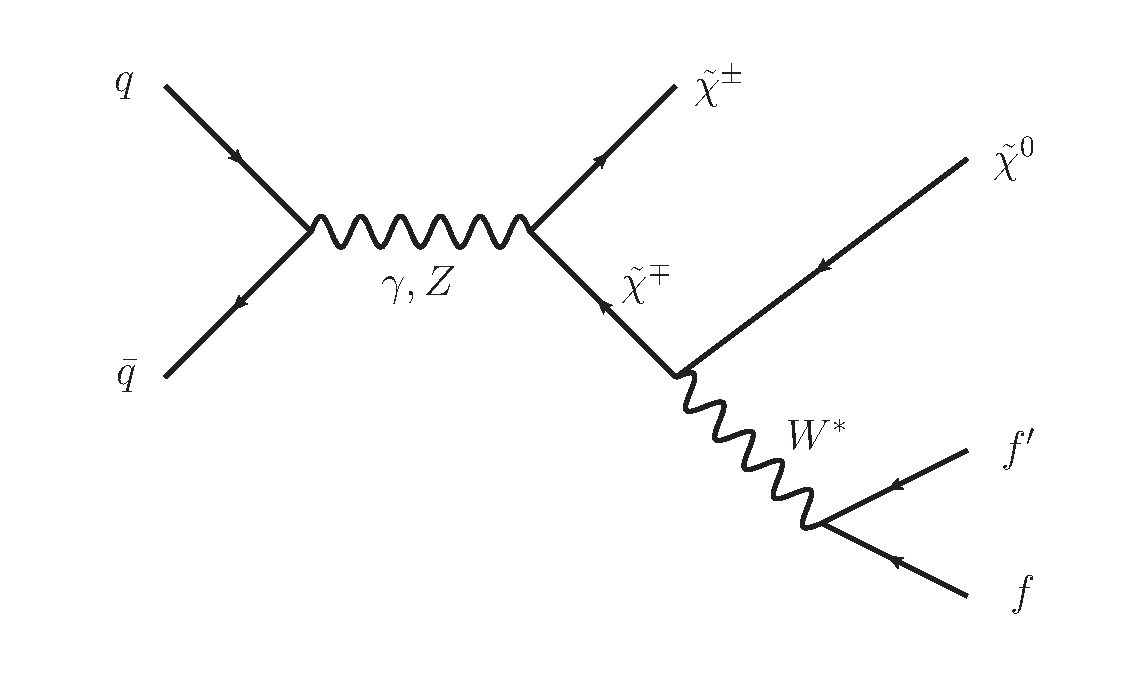
\includegraphics[width=0.75\textwidth]{figures/analysis/ChiChi_ProductionAndDecay.pdf}
  \end{tabular}
  \caption{Feynman diagram showing a possible production mechanism of a chargino pair and the decay channel of a chargino.}
  \label{fig:FeynmanDiagram}
\end{figure}

Other possible production channels are the exchange of a supersymmetric Higgs boson or via a t-channel squark exchange. 
The corresponding Feynman diagrams for the tree level production channels are shown in Fig.~\ref{fig:FeynmanDiagramProductionCharginoPair}.

\begin{figure}[!t]
  \centering 
  \begin{tabular}{c}
    \frame{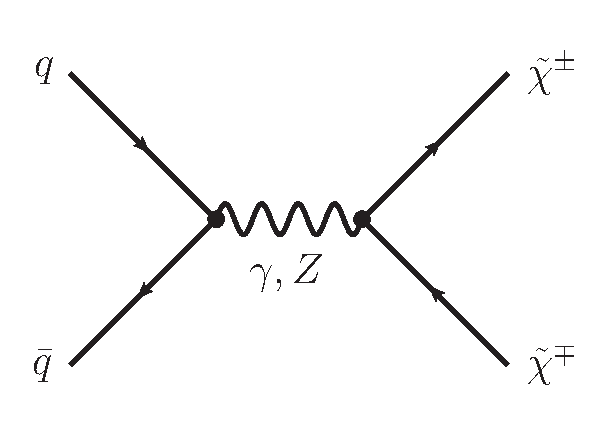
\includegraphics[width=0.33\textwidth]{figures/analysis/ChiChi_GammaZ.pdf}
    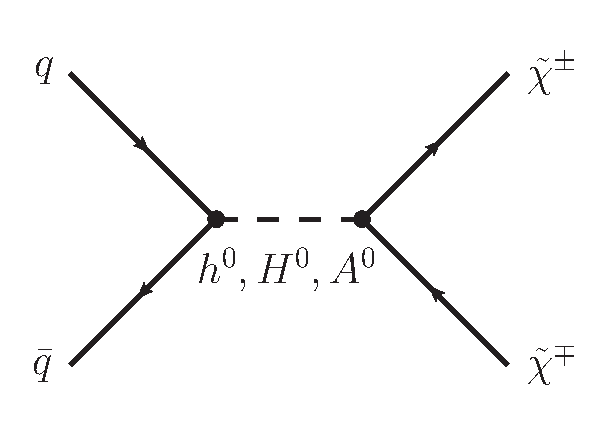
\includegraphics[width=0.33\textwidth]{figures/analysis/ChiChi_Scalar.pdf}
    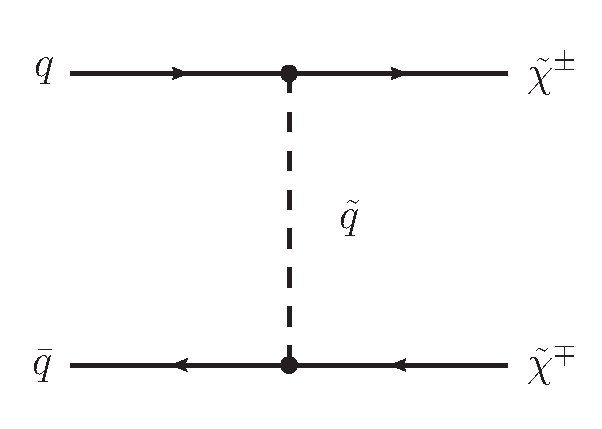
\includegraphics[width=0.33\textwidth]{figures/analysis/ChiChi_Squark.pdf}}
  \end{tabular}
  \caption{Main tree level diagrams for chargino pair production.}
  \label{fig:FeynmanDiagramProductionCharginoPair}
\begin{tabular}{c}
    \frame{    
    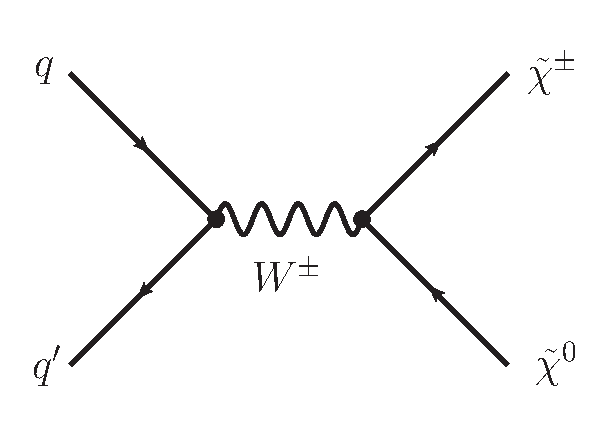
\includegraphics[width=0.33\textwidth]{figures/analysis/ChiChi0_WBoson.pdf}
    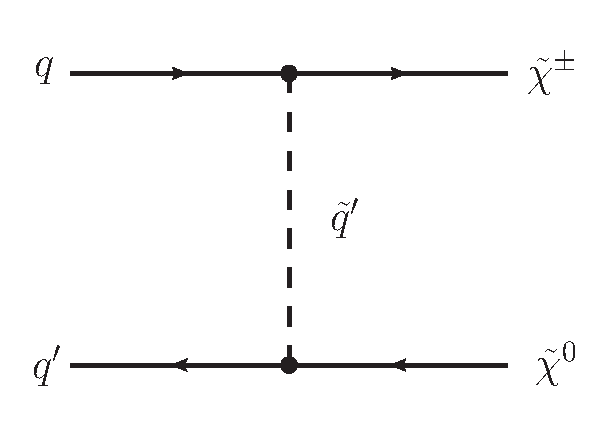
\includegraphics[width=0.33\textwidth]{figures/analysis/ChiChi0_Squark.pdf}
    }
  \end{tabular}
  \caption{Main tree level diagrams for chargino neutralino production.}
  \label{fig:FeynmanDiagramProductionCharginoNeutralino}
\end{figure}
Another possibility of chargino production is the chargino neutralino production channel. 
On tree level, there exist two production mechanism: the s-channel W boson exchange and the t-channel squark exchange, see Fig.~\ref{fig:FeynmanDiagramProductionCharginoNeutralino} for the Feynman diagrams.\\

Even if the presented supersymmetric model where $\chi^{\pm}_1$ and $\chi^{0}_1$ are nearly mass-degenerate leads to more exotic signatures at the CMS experiment, there have been already several analyses conducted in CMS which are in principle (even not all were designed to be) sensitive to these models.
Among those are a search for long-lived charged particles \cite{bib:CMS:HSCP_8TeV}, which was mainly designed for particles which have such a long lifetime that they travel through the full detector without decaying and a search for disappearing tracks \cite{bib:CMS:DT_8TeV} which looked for rather intermediate lifetimes, where the charginos decays already inside the tracker. 
Within \cite{bib:CMS:DT_8TeV}, a study was done, based on an interpretation exercise \cite{bib:CMS:HSCPReinterpreation_PAS} within the phenomenological MSSM (see Sec.~\ref{theorySUSY} for a detailed introduction to the pMSSM), which tests the exclusion power of various analyses done at CMS.

\begin{figure}[!t]
  \centering 
  \begin{tabular}{c}
    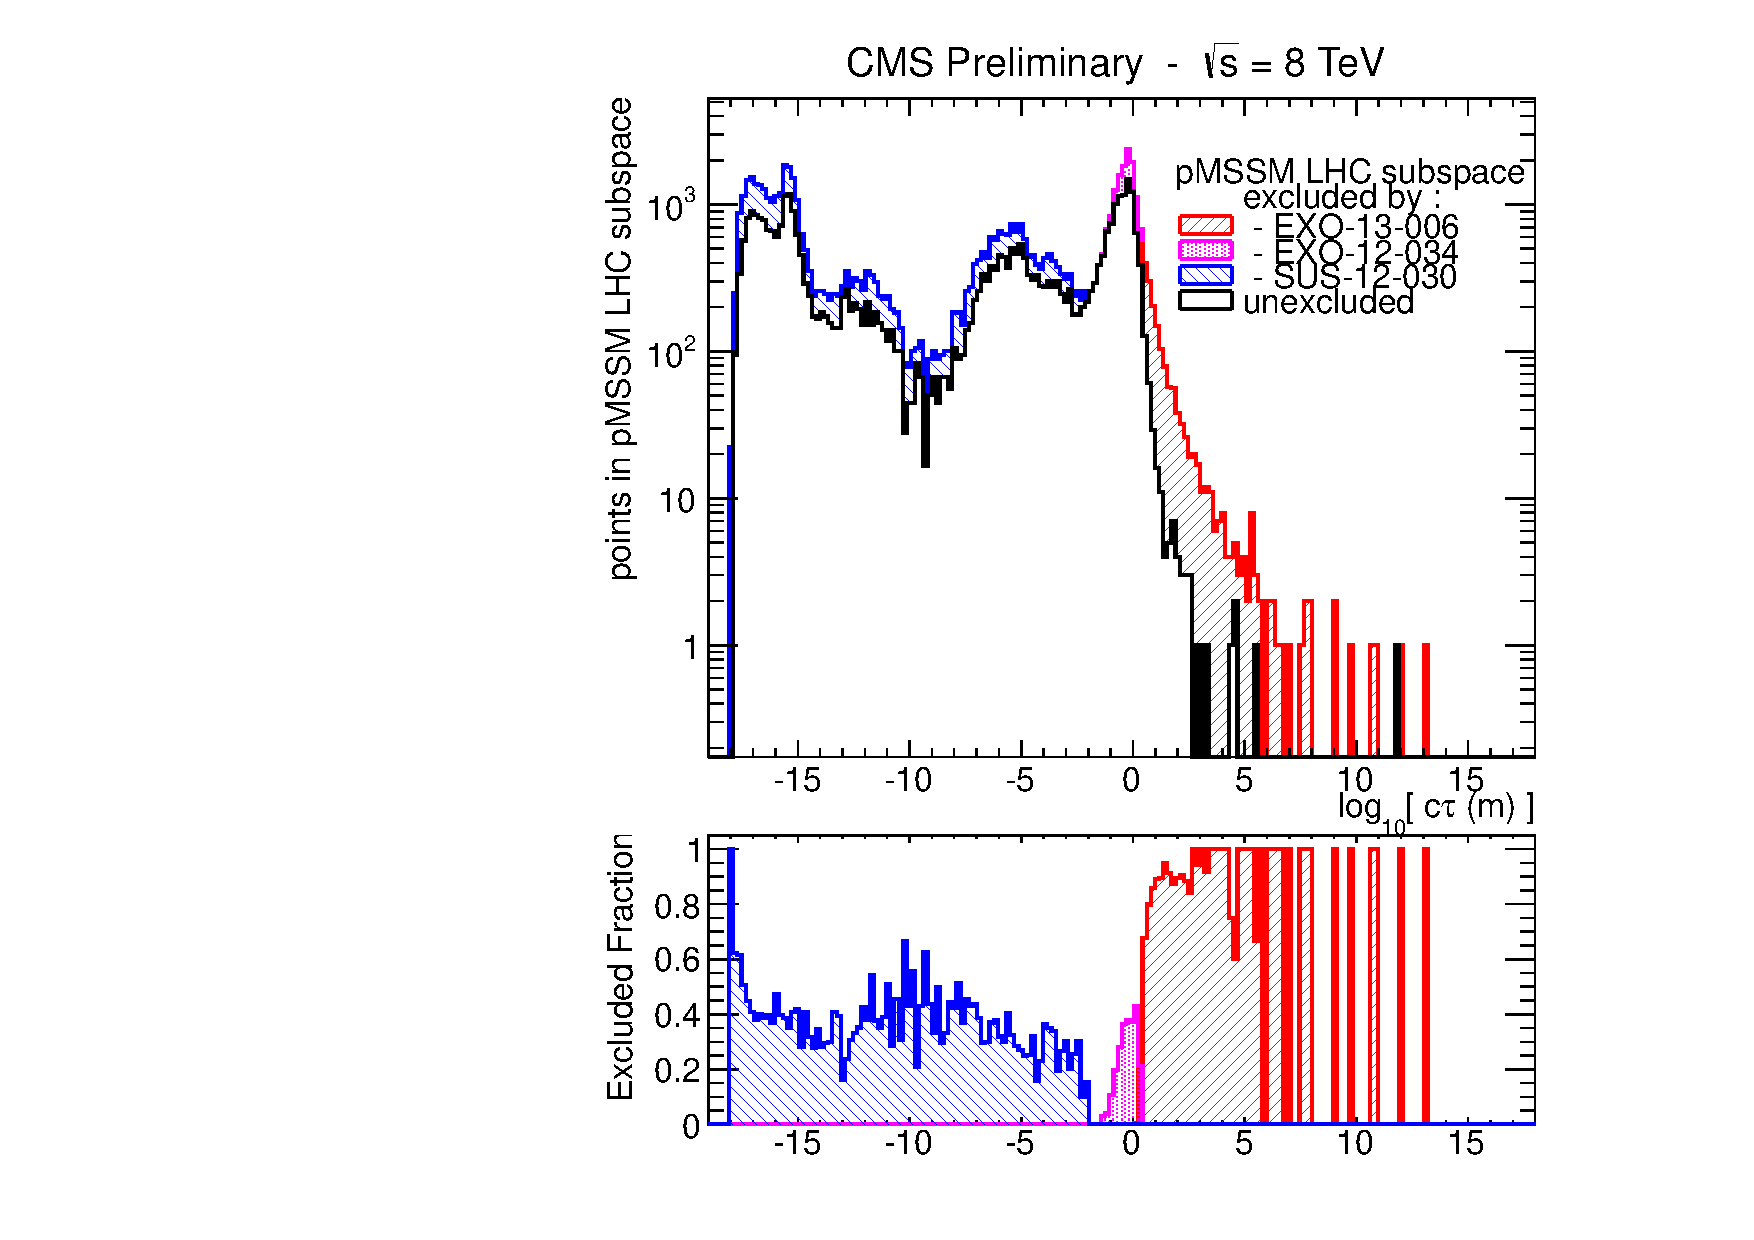
\includegraphics[width=0.75\textwidth]{figures/analysis/pMSSM_vs_ctau.pdf}
  \end{tabular}
  \caption{Exclusion power of various analyses dependent on chargino lifetime [c$\tau$]. Lower part of the plot shows the excluded fraction. Taken from: \href{https://twiki.cern.ch/twiki/bin/view/CMSPublic/PhysicsResultsEXO12034}{click here}.}
  \label{fig:pMSSMplot}
\end{figure}
In Fig.~\ref{fig:pMSSMplot}, the exclusion power of the search for long-live charged particles \cite{bib:CMS:HSCP_8TeV} in red, the search for diasappearing tracks \cite{bib:CMS:DT_8TeV} in purple and a collection of various SUSY analysis from \cite{bib:CMS:pMSSMinterpretation_7TeV_PAS} in blue over the chargino mass is shown. 
In black the distribution of the unexcluded pMSSM parameter points vs. the chargino lifetime can be seen.
The sampling of the parameter space points was done according to a pre-CMS likehood function, which takes into account electroweak precisicion measurements, etc.
In the lower part of Fig~\ref{fig:pMSSMplot}, the excluded fraction of pMSSM points is shown. 
It can be seen, that the more general SUSY searches are mostly sensitive to shorter chargino lifetimes ($c\tau \lesssim 10 \,\text{cm}$)\footnote{It should be mention, that because the inpossibility of simulating long-lived charginos in from the generator, it could not be tested to which exact upper lifetime, the searches are sensitive. But it is reasonable to argue, that they won't be sensitive to longer lifetimes, as these are usually high backgorund searches}, whereas the search for long-lived particles shows very good sensitivity for lifetimes $>100\,$cm.
The search for disappearing tracks is sensitive on supersymmetric models with chargino lifetimes between $35\,\text{cm} \lesssim c\tau \lesssim 100\,\text{cm}$.

This analysis is targeting the gap between the disappearing track search (purple area) and the searches which are sensitive to instanteanously decaying charginos (blue area). 
The idea is to make use of the variable dE/dx which can be very discriminating for particles with high mass.
The challenges of such a search and the general strategy of this analysis will be presented int the next section.

%%%%%%%%%%%%%%%%%%%%%%%%%%%%%%%%%%%%%%%%%%%%%%%%%%%%%%%%%%%%%%%%%%%%%%%%%%%%%%%%%%%%%%%%%%%%%%%%%%%%%%%%%%%%%%%%%%%%%%%%%%%%%%%%%%%%%%%%%%%%%%%%%%%%%%%%%%%%%%%%%%%%%%%%%%%%%%%%%%%%
%%%%%%%%%%%%%%%%%%%%%%%%%%%%%%%%%%%%%%%%%%%%%%%%%%%%%%%%%%%%%%%%%%%%%%%%%%%%%%%%%%%%%%%%%%%%%%%%%%%%%%%%%%%%%%%%%%%%%%%%%%%%%%%%%%%%%%%%%%%%%%%%%%%%%%%%%%%%%%%%%%%%%%%%%%%%%%%%%%%%
\section{General search strategy}
\label{sec:GeneralSearchStrategy}

When searching for supersymmetric models with long-lived \chipm, the strategy is of course highly dependent on the actual lifetime of the chargino. 
For long lifetimes, the chargino can reach the muon chambers and can be reconstructed as a muon (even with a longer time-of-flight). 
For lower lifetimes, the chargino can already decay inside the detector (e.g. the tracker), thus not leading to a reconstructed muon in the event, but only to an isolated track in the tracker. 
The detector signatures of these two scenarios are visualised in Fig~\ref{fig:CharginoPaiEventDisplay}, where in a cross-sectional view of the CMS detector simulated chargino-chargino events are shown.
\begin{figure}[!t]
  \centering 
  \begin{tabular}{c}
    \frame{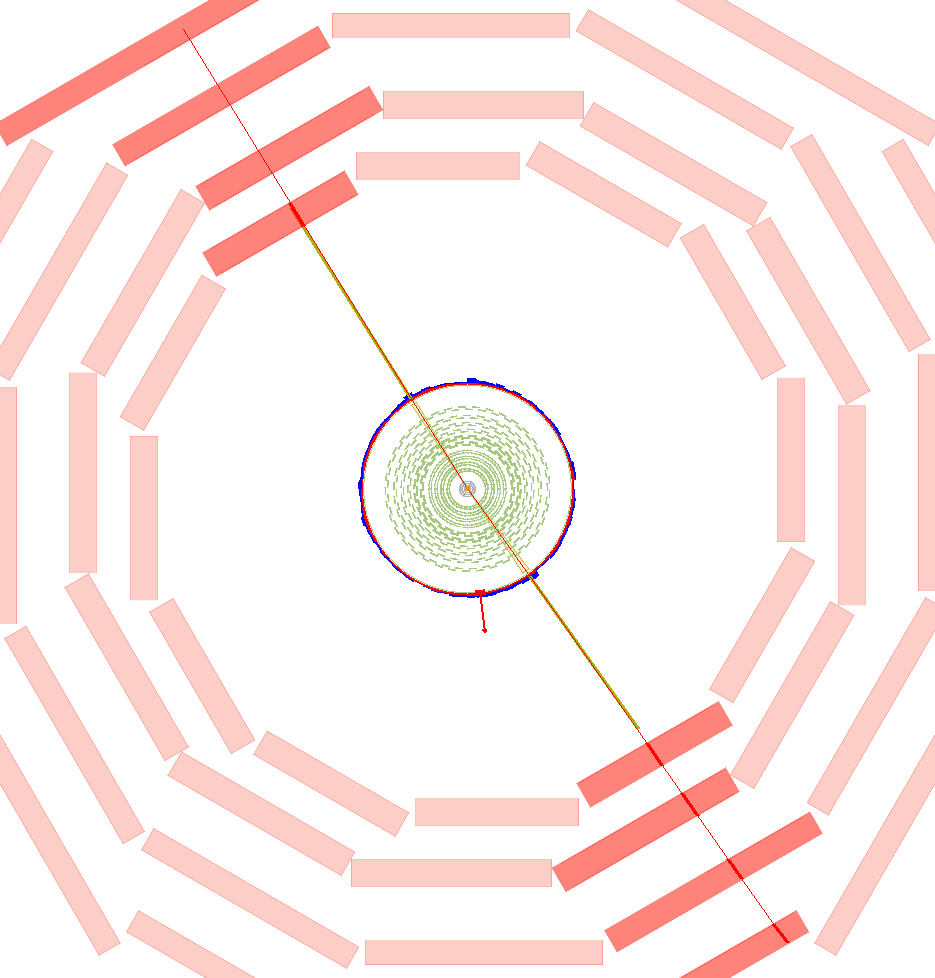
\includegraphics[width=0.31\textwidth]{figures/analysis/EventDisplay_scenario1.png}}
    \frame{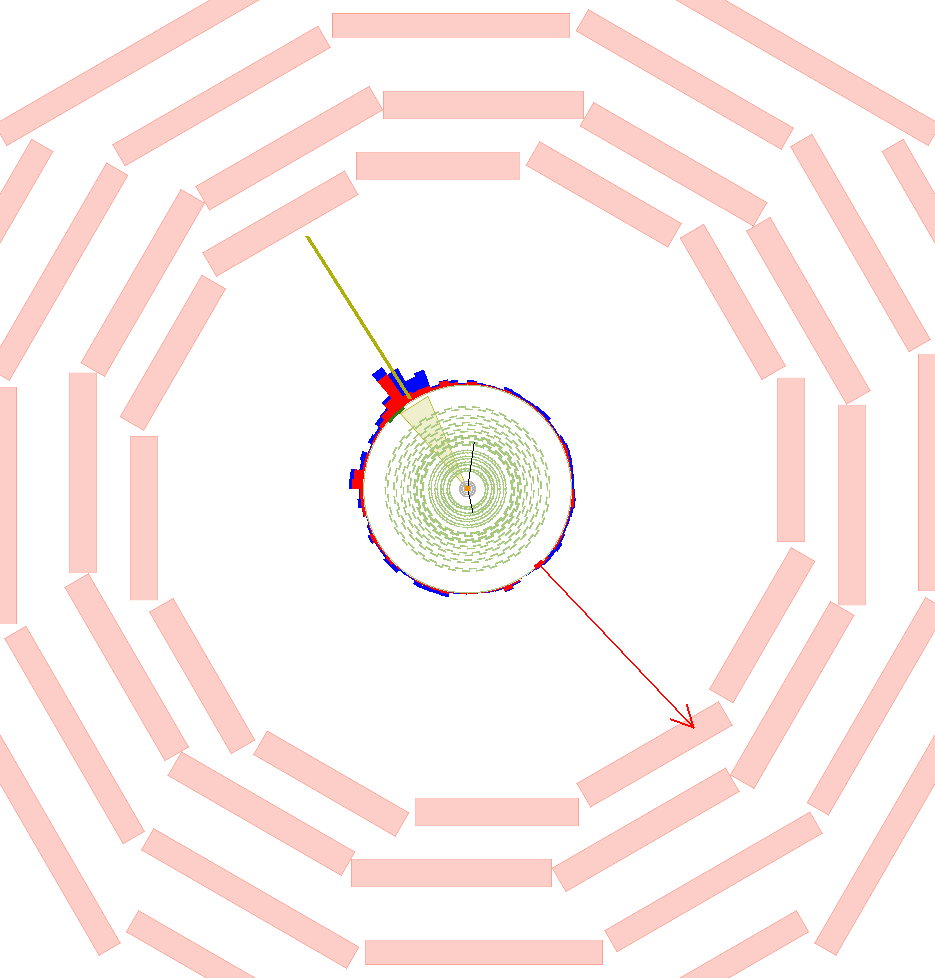
\includegraphics[width=0.31\textwidth]{figures/analysis/EventDisplay_scenario2.png}}
    \frame{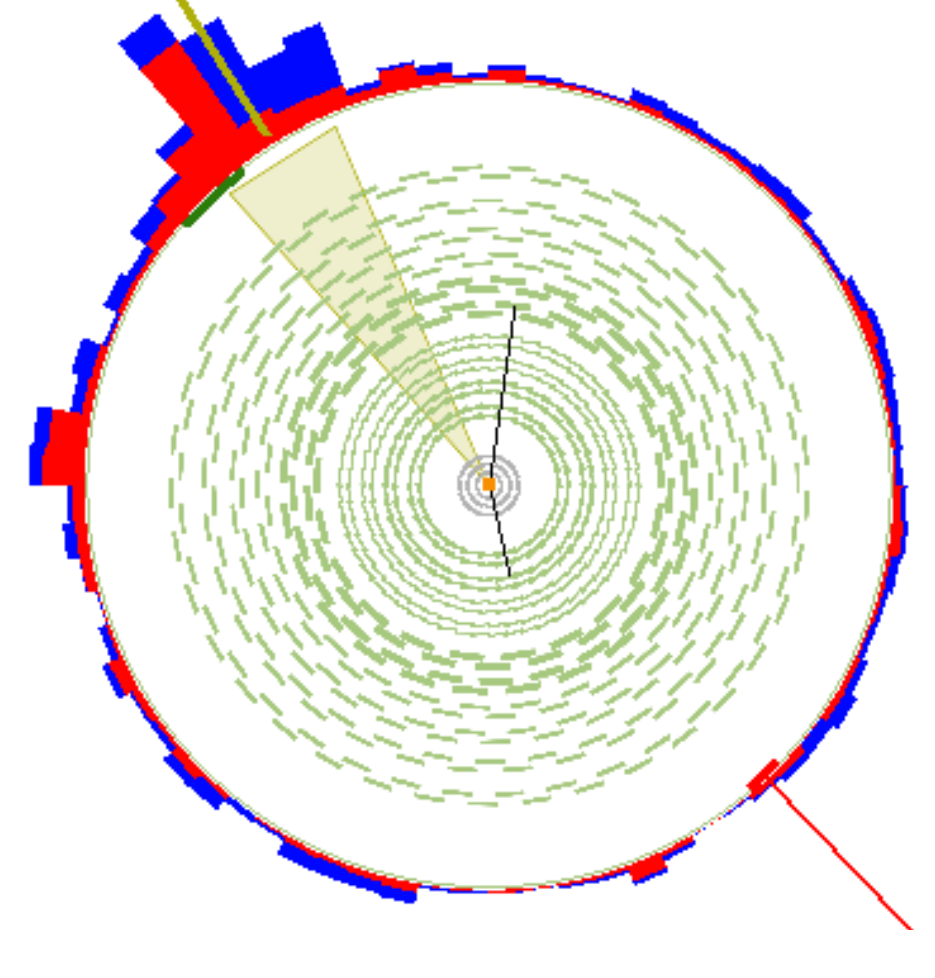
\includegraphics[width=0.31\textwidth]{figures/analysis/EventDisplay_scenario2_Zoomed.png}}
  \end{tabular}
  \caption{Visualisation of possible signatures of a chargino pair produced with a lifetime of $c\tau = 10\,\text{m}$ (left) and a lifetime of $c\tau = 0.5\,\text{m}$ (middle and right). 
           In the left picture, both charginos are reconstructed as muons, which can be seen in the energy deposition in the muon chambers (red boxes). 
           In the middle picture both charginos are only visible as tracks in the tracker (black lines), where both trajectories end inside the silicon tracker, showing the decay point point of the corresponding chargino. 
           The right picture is a zoom of the picture in the middle. Here only the cross-section of the tracker (green wavy lines) is displayed. The red arrow shows the missing transverse energy in the event.} 
  \label{fig:CharginoPaiEventDisplay}
\end{figure}
As mentioned before, this analysis targets a search for supersymmetry with charginos of lifetimes between $10\,\text{cm} \lesssim c\tau \lesssim  40\,\text{cm}$.
That means that the charginos decay rather early in the detector, even at the beginning of the tracker. 
The distinct challenges of such an analysis, shall be listed in the following passage.

First of all, in case R-parity (see Sec.~\ref{theorySUSY}) is conserved, one of the decay products of the chargino, which is the lightest neutralino \chiO is stable, thus travelling through the whole detector only weakly intereacting.
Therefore it is not detectable. 
The other chargino decay product, e.g. a pion, can be hardly reconstructed, mainly because it does not origin from the primary vertex (if the chargino reaches the detector before its decay), 
but secondarily because it is very low in momentum because of the mass-degeneracy between \chipm and \chiO.
The momentum of the decay product is of course highly dependent on the actual mass gap between the neutralino and the chargino.
The typical momentum of a pion originating from a chargino to neutralino decay is in the \chipm rest frame of the order 
\begin{equation*}
p_{\pi}\sim \sqrt{m_{\chi^{\pm}_1}-m_{\chi^{0}_1}-m_{\pi}}.
\end{equation*}
%As the \chipm is rather slow for higher masses this is a good approximation also in the detector rest frame.
A \pt distribution of the pion for a simulation with $\sqrt{s} = 8\,\tev$ can be found in Fig.~\ref{fig:KinkedTrack} for a mass gap between \chipm and \chiO of $\Delta m=150\, \mev$.
\begin{figure}[!b]
  \centering 
  \begin{tabular}{c}
    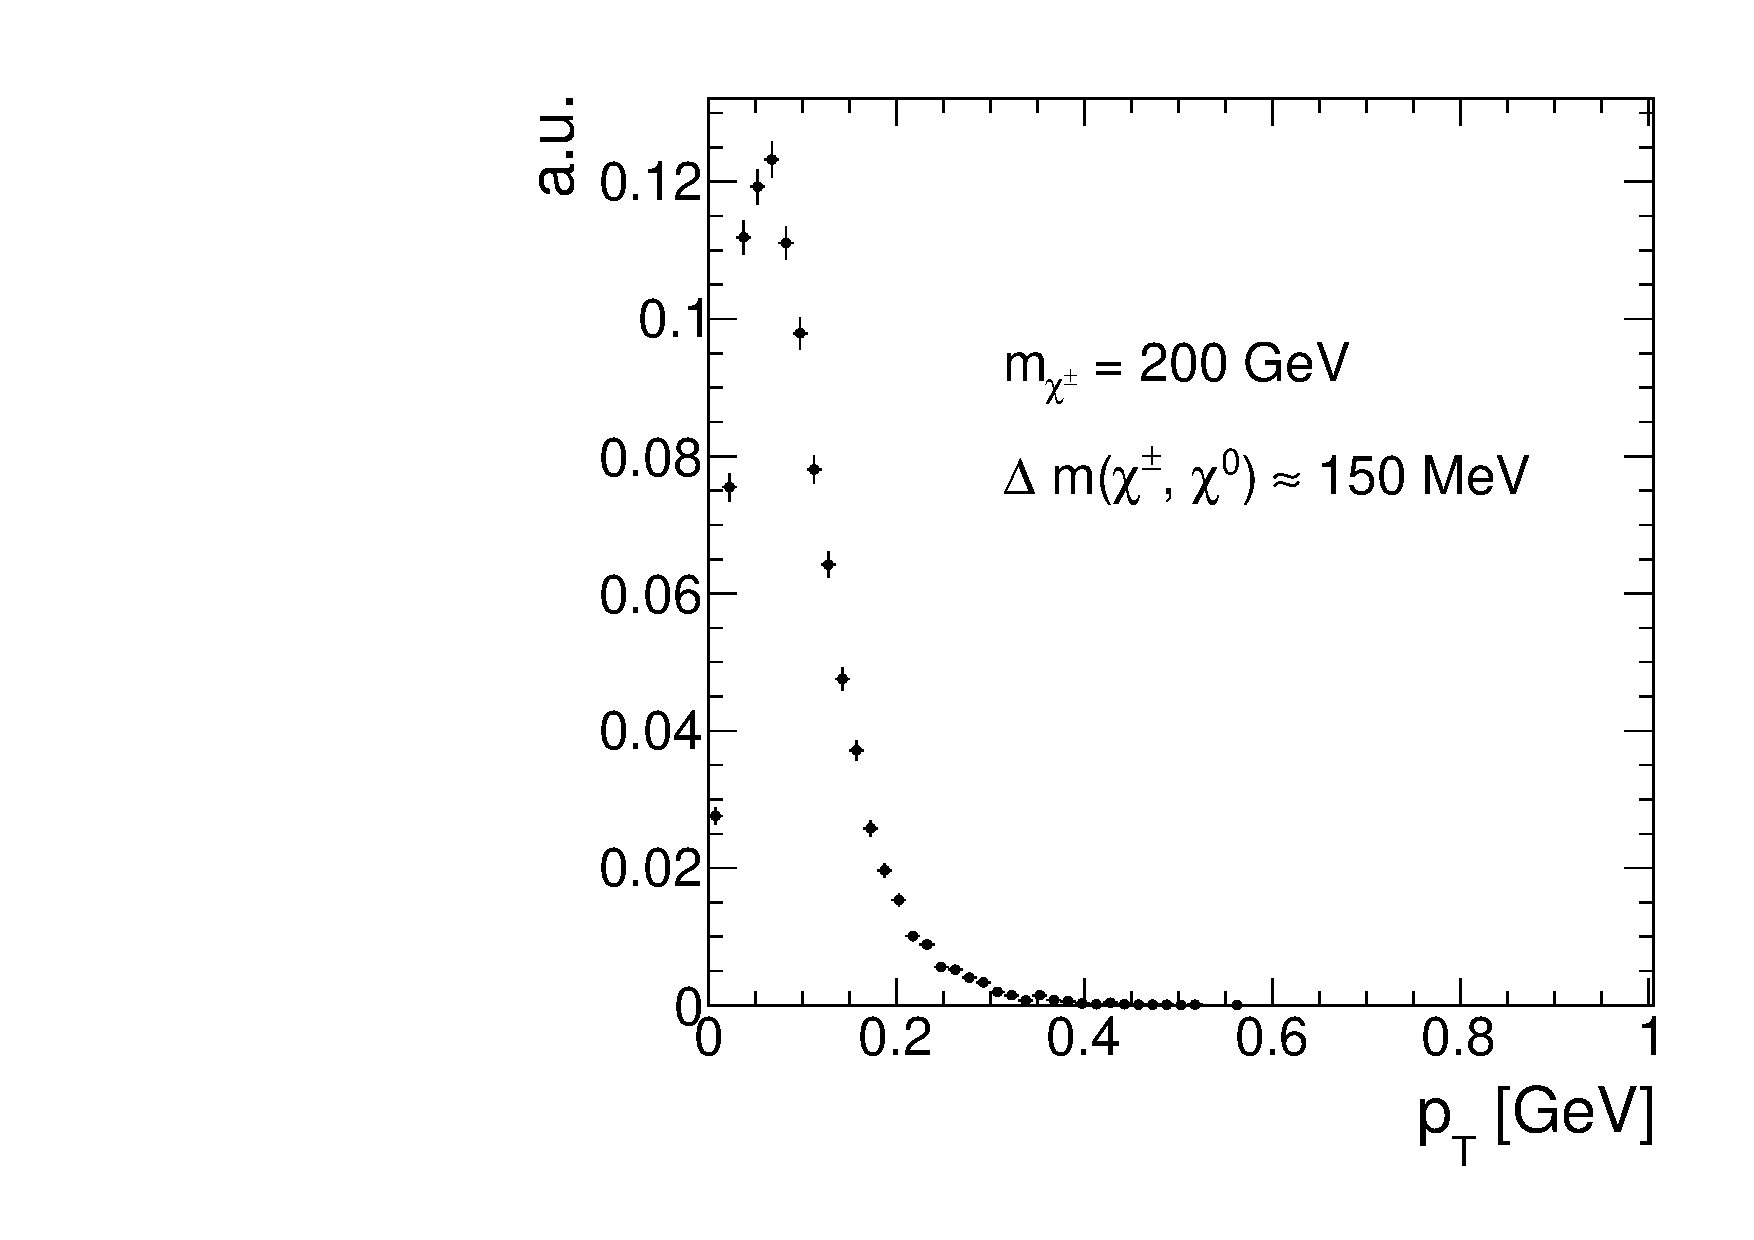
\includegraphics[width=0.49\textwidth]{figures/analysis/PtOfPions.pdf}
  \end{tabular}
  \caption{Transverse momentum distribution of pions coming from chargino decay into a neutralino with a mass gap of 150\mev.}
  \label{fig:ptOfPions}
\end{figure} 
The \pt distribution peaks \mbox{at $\sim$ 100\,\mev} and ends at \mbox{\pt $\sim 400\,$\mev}.
When the transverse momentum of a particle is very low, the particle trajectory is much more bended compared to a particle with higher \pt (see Fig.~\ref{fig:KinkedTrack} for illustration), 
thus making the detection of such a particle very challinging.
\begin{figure}[!bt]
  \centering 
  \begin{tabular}{c}
    \frame{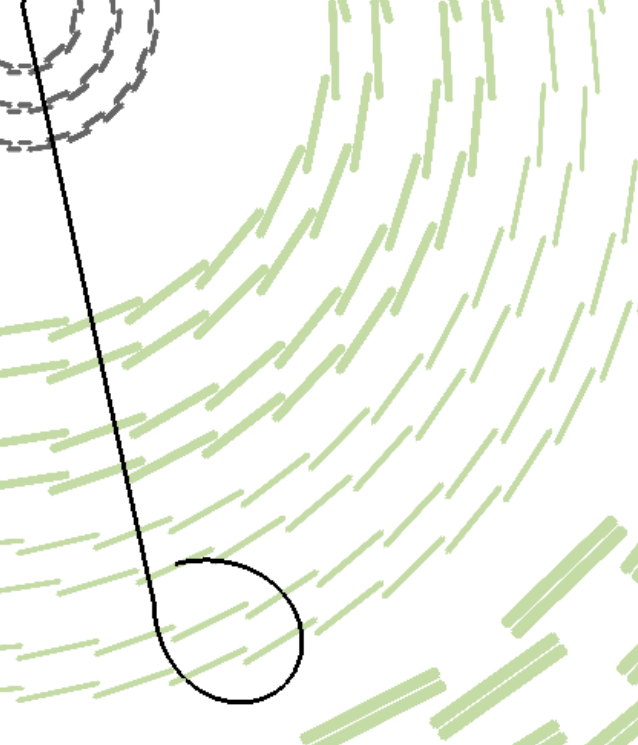
\includegraphics[width=0.3\textwidth]{figures/analysis/KinkedTrackZoom.png}}
  \end{tabular}
  \caption{Cross-sectional view of the tracker (different tracker layers are illustrated with wavy green lines) and a simulated chargino track (black line) decays to a pion (bended black line).}
  \label{fig:KinkedTrack}
\end{figure} 
Because of the stronger bending, the track reconstruction efficiency decreases for particles with a transverse momentum below 1\,\gev rapidely, ending at around 40\% for isolated pions with a \pt of 100\mev (see \cite{bib:CMS:tracking_8TeV}).

Taking the hard or even impossible detection of the decay products of the chargino, this lead to the fact, that besides the (short) track of the chargino, nothing can be seen in the detector.
Unfortunately, there is no dedicated track trigger at CMS, which makes a specific detection of those events with the help of the chargino track impossible.
To be able to search for these models, one therefore needs to take advantage of higher order contributions to the feynman diagrams shown in the previous sections (Figs.~\ref{fig:FeynmanDiagramProductionCharginoPair},\ref{fig:FeynmanDiagramProductionCharginoNeutralino}), resulting in initial state radiation (ISR).
When the initial quarks radiate a high \pt gluon, the resulting jet can be detected and can offer a possibility to search for isolated tracks in the tracker.
The non-detection of the chargino's decay products plus a high \pt ISR jet lead additionally to missing transverse energy (MET) in the event. 
Exploiding these two circumstances, it is possible to detect chargino-pair or chargino-neutralino events with the help of Jet+MET triggers.

To select possible charginos in an event, additional requirements for isolated, high \pt tracks are needed.
Those tracks can be eventually disappearing, which means that the track does not cross the full pixel and strip detector.
This can happen, when the chargino decays inside the tracker.
For very low lifetimes, the tracks can be very short and can have only a few hits in the detector. 
To define a helical path five parameters are needed, therefore a minimum of three hits are required to be able to reconstruct a particle's trajectory (see \cite{bib:CMS:tracking_8TeV}).
In this analysis, the massiveness of the charginos shall be exploited, on the one hand by selecting only high \pt tracks, but on the other hand by requiering a high energy deposition per path length (\dedx).
The energy deposition depends quadratically on the particle's mass for low velocities ($0.2<\beta\gamma<0.9$).
\begin{equation*}
\langle\frac{dE}{dx}\rangle = K \frac{m^2}{p^2} +C
\end{equation*}
thus constitute a very nice discriminating variable for massive particles against SM particles.
 
A specific challenge for this analysis is hence the combination of searching for short tracks and utilising the measurement of the energy deposition of the chargino.
For a short track, eventually only passing the first couple layers of the whole tracker system, the pixel tracker becomes obviously very important.
This means that a good energy measurement in the pixel system is of great importance to this analysis.
However, no other CMS analysis used the energy information of the pixel tracker so far.
That means, that a thoroughly study of the quality of the pixel energy calibration needs to be undertaken, and in case the energy calibration is not suffiencient, a further energy calibration needs to be carried out.


\subsection{Comparison to existing searches}
As already mentioned before, there are several analyses at CMS at $\sqrt{s}=8\,\tev$ with 20\,fb$^{-1}$ data, which are sensitive to intermediate lifetime charginos. 
Most notably, the search for long lived-charged \mbox{particles \cite{bib:CMS:HSCP_8TeV}} and the search for disappering tracks \cite{bib:CMS:DT_8TeV}.
An improvement in sensitivity to shorter lifetimes compared to these analysis shall be achieved in a twofold way:
First, the selection in this analysis shall also include very short tracks.
And secondly, also the inclusion of the variable \dedx as discriminating variable shall increase the search sensitivity compared to \cite{bib:CMS:DT_8TeV}.

In \cite{bib:CMS:HSCP_8TeV}, for every track a minimum number of eight hits, whereas in \cite{bib:CMS:DT_8TeV} a minimum of seven hits were required. 
This can be very unefficient for shorter lifetimes, where most of the charginos decay already shortly after the pixel tracker.

Additionally, the search for disappearing tracks (which targets models with charginos decaying inside the tracker) did not make use of the high energy deposition of heavy particles. 
Although this variable was indeed used in the search for long-lived particles, this search was not especially designed for intermediate lifetimes (e.g. no muon veto on the selected tracks was required), 
thus it shows less sensitivity compared to the disappearing track search in the lifetime region between $35\,\text{cm} \lesssim c\tau \lesssim 100\,\text{cm}$ (see Fig~\ref{fig:pMSSMplot}).

Therefore, the general search strategy of the preseneted analysis is to unite the strategies of \cite{bib:CMS:HSCP_8TeV} and \cite{bib:CMS:DT_8TeV} and to lower the strong selection on the number of hits in these analyses 
to get an optimized selection for lifetimes around $10\,\text{cm} \lesssim c\tau \lesssim  40\,\text{cm}$.


\textcolor{red}{MAYBE} show here already a plot with the number of valid hits distribution to emphasize the importance of lossening the number of hits cut!
%%%%%%%%%%%%%%%%%%%%%%%%%%%%%%%%%%%%%%%%%%%%%%%%%%%%%%%%%%%%%%%%%%%%%%%%%%%%%%%%%%%%%%%%%%%%%%%%%%%%%%%%%%%%%%%%%%%%%%%%%%%%%%%%%%%%%%%%%%%%%%%%%%%%%%%%%%%%%%%%%%%%%%%%%%%%%%%%%%%%
%%%%%%%%%%%%%%%%%%%%%%%%%%%%%%%%%%%%%%%%%%%%%%%%%%%%%%%%%%%%%%%%%%%%%%%%%%%%%%%%%%%%%%%%%%%%%%%%%%%%%%%%%%%%%%%%%%%%%%%%%%%%%%%%%%%%%%%%%%%%%%%%%%%%%%%%%%%%%%%%%%%%%%%%%%%%%%%%%%%%
\section{Improved dE/dx measurement of short tracks}
\label{sec:DeDxMeasurement}
It was already pointed out, that the inclusion of the pixel energy measurements can increase the sensitivity when searching for short tracks.
While the silicon strip detector has already been calibrated as part of the search for long-lived charged particles \cite{bib:CMS:HSCP_8TeV}, there was never an offline calibration done for the pixel silicon tracker.
To increase the discrimination power of $dE/dx$, such an calibration procedure was therefore conducted within this PHD thesis.
 
\subsection{Measuring dE/dx}
\label{sec:sub:MeasuringDeDx}
The mean energy loss per path length of particles travelling through a layer of material can be described with the Bethe formula \cite{bib:Bethe_1930}:
\begin{equation*}
\langle \frac{dE}{dx} \rangle = kz^2\frac{Z}{A}\frac{1}{\beta^2} [ \frac{1}{2} \ln{\frac{2m_e c^2 \beta^2 \gamma^2 T_{\text{max}}}{I^2}} - \beta^2 - \frac{\delta( \beta \gamma )}{2} ].
\end{equation*}
It is valid, where the main energy loss originates from ionization effects, i.e. in a region between $0.1\lesssim\beta\gamma\lesssim 1000$.
It is a function of the atomic number ($Z$) and the atomic mass of the absorber ($A$). 
The mean excitation energy ($I$) for silicon is 173\,eV \cite{bib:NIST}. 
$T_{\text{max}}$ stands for the maximum energy transfer in a single collision.
The relevant particle's properties are the velocity ($\beta$), the lorentz factor ($\gamma$) and the charge (z) of the incident particle.
The density correction $\delta( \beta \gamma )$ reduces the mean energy loss at high energies because of polarization effects of the material.

Even if widely used, the mean energy loss is a quantity which is ``ill-defined experimentally and is not useful for describing energy loss by single particles'' \cite{bib:PDG_2014}.
The problem is caused by the underlying probability distribution of one single $dE/dx$ measurement (this will be named by $\Delta E/ \Delta x $ throughout the following sections), which can be parametrized by a Landau distribution \cite{bib:Landau_1944}
\begin{equation*}
p(x) = \frac{1}{\pi} \int_0^\infty\! e^{-t \log t - x t} \sin(\pi t)\, dt.
\end{equation*}
The Landau distribution is a highly asymmetric distribution with a long tail torwards the right end (see Fig.~\ref{fig:landau}).
Theoretically it extends to infinite energies, however in nature the maximal deposited energy is of course limited by the particle's full energy.
\begin{figure}[!t]
  \centering 
  \begin{tabular}{c}
  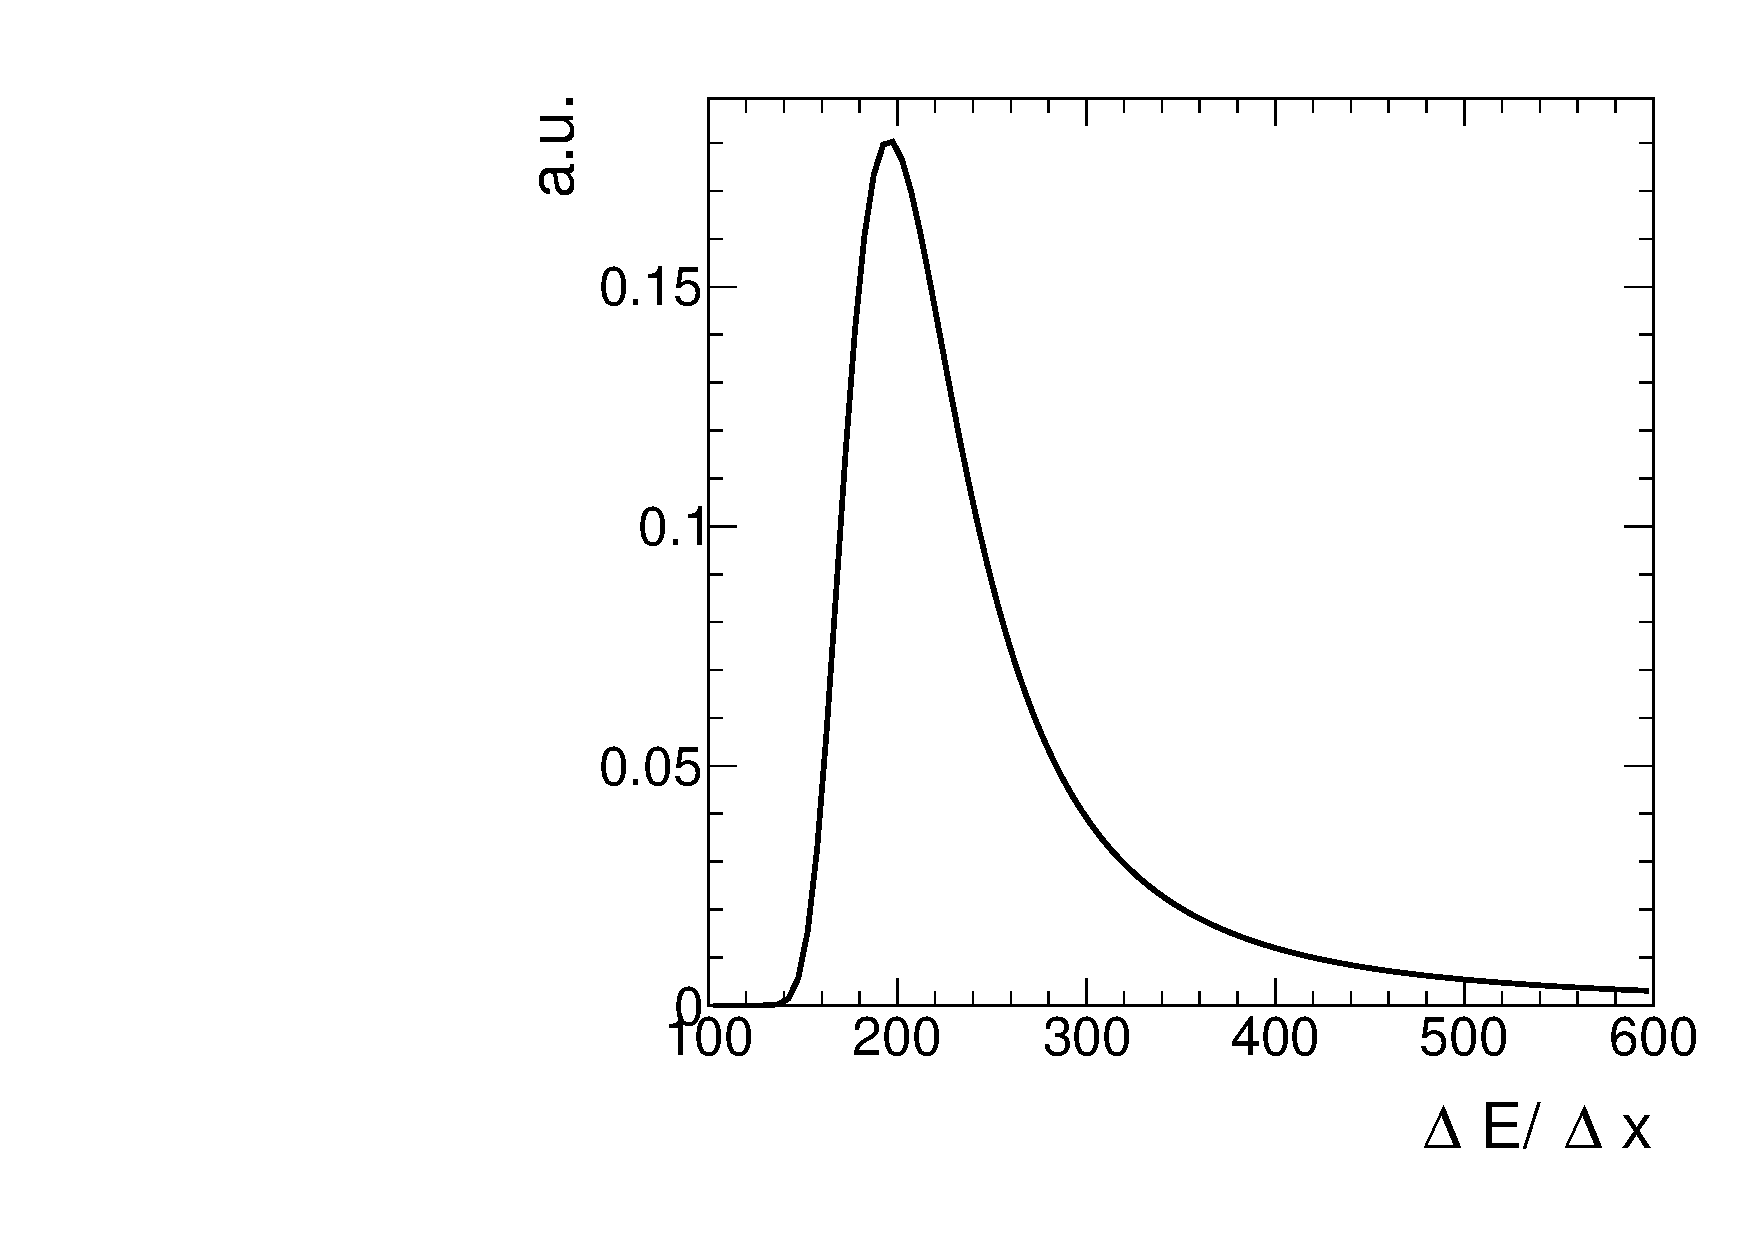
\includegraphics[width=0.49\textwidth]{figures/analysis/Landau.pdf}
  \end{tabular}
  \caption{Illustration of the shape of a Landau function. Parameters were arbitrarily chosen for this figure.} 
  \label{fig:landau}
\end{figure}
The mean and the variance of a landau distribution are not defined.
Because of its high assymetry, measurements of $\langle dE/dx \rangle$ with only a few single measurements are easily biased torwards high values, making the mean energy loss described by the Bethe formula to a problematic and unstable concept. 
%This is again different for a (limited) measurment, as there it is always possible to calucalute a mean.
%Still, this leads to the fact that the definition of the mean energy loss per path length is a problematic and unstable concept.


A much better observable is the most probably value (MPV): the maximum of the Landau function.
The MPV is much more stable compared to the mean and is not as easily biased towards higher $dE/dx$ values. 
The most probable energy loss of a charged particle is defined by the Landau-Vavilov-Bichsel equation \cite{bib:Bichsel:MPV_1988}:
\begin{equation}
\Delta_p = \xi \left[ \ln \frac{2mc^2\beta^2\gamma^2}{I}  + \ln\frac{\xi}{I} + j - \beta^2 - \delta(\beta\gamma)  \right],
\label{eq:Landau_Vavilov_Bichsel}
\end{equation}
with $\xi=(K/Z)\langle Z/A \rangle (x/\beta^2)$. 
The thickness of the absorber $x$ appears explicitly in the Landau-Vavilov-Bichsel equation making the most probable energy loss per path \mbox{length $\Delta_p/dx$} logarithmically dependent on $x$.
A comparison between the Bethe mean energy loss $\langle dE/dx \rangle$ and the most probable energy loss $\Delta_p/dx$ is shown in Fig.~\ref{fig:dEdx_Bethe_Landau}.
\begin{figure}[!bt]
  \centering 
  \begin{tabular}{c}
  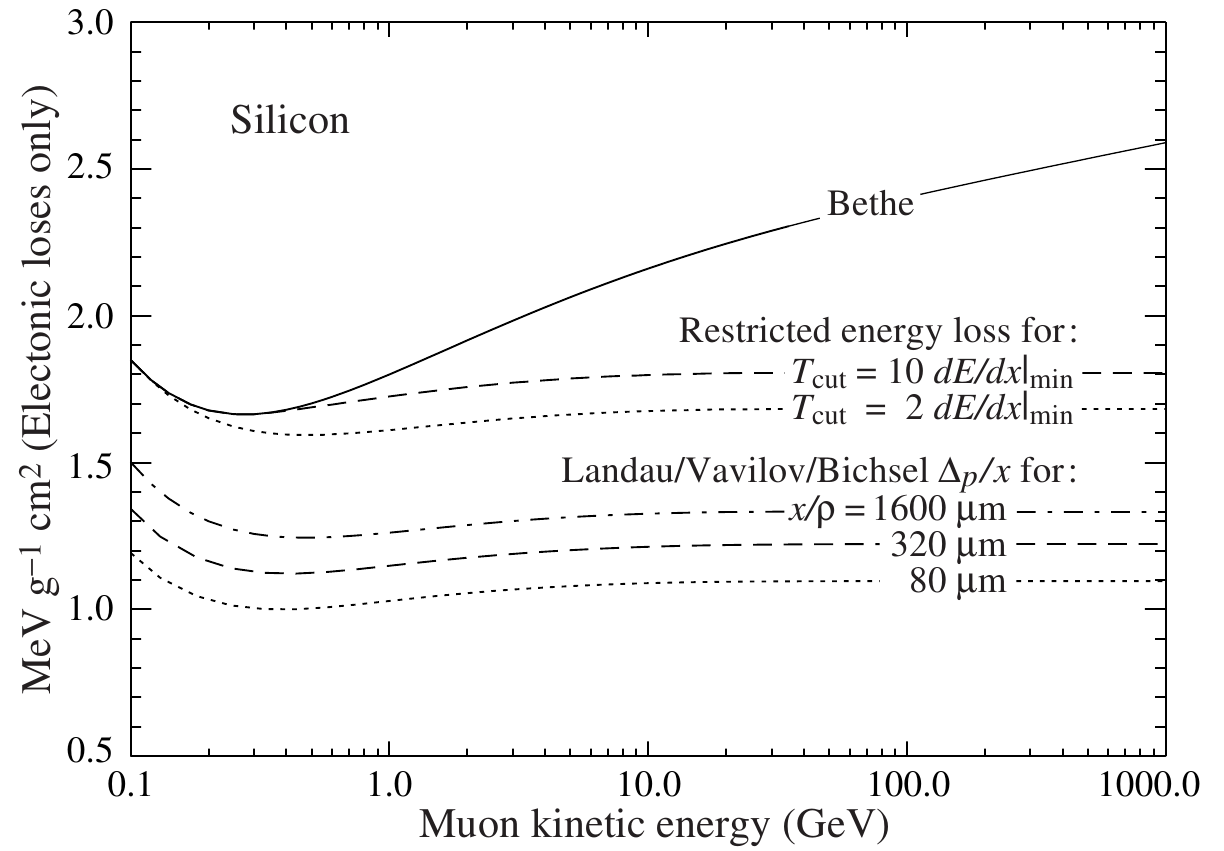
\includegraphics[width=0.6\textwidth]{figures/analysis/dEdx_Bethe_Landau.png}
  \end{tabular}
  \caption{Comparison between the Bethe mean energy loss with and without restricted energy loss and the most probable energy loss described by the Landau-Vavilov-Bichsel function for different sizes of thickness. 
           Taken from \cite{bib:PDG_2014}.} 
  \label{fig:dEdx_Bethe_Landau}
\end{figure}
However, when measureing tracks with around $\sim$15 hits, it is obviously not too simple to extract the most probable value. 
Large fluctuations can still lead to biases towards higher value of the most probable $dE/dx$.

There are several "estimators'', which try to suppress as much as possible a bias towards the high end, without introducing a bias to lower values.
One of the estimator, also used in the next chapter, is the harmonic-2 estimator

\begin{equation}
I_{h2}=\left( \frac{1}{N}\sum_{i=1}^{N}(\Delta E/\Delta x)_i^2 \right)^{-1/2},
\label{eq:Harmonic2Estimator}
\end{equation}
where $\Delta E /\Delta x$ correspond to one measurement in one tracker module. 
The harmonic mean of all $N$ measurements with the power of 2 is then the estimated most probable $dE/dx$.\\

SM particles as pions and muons are minimal ionising in silicon for $\beta\gamma \sim 4$ (see Fig.~\ref{fig:dEdx_Landau_Silicon}). 
For higher momenta the deposited energies increase again reaching a plateau at around $\beta\gamma\sim100$. 
However, new heavy charged particles would mainly be unrelativistic because of their high mass and would therefore deposit much higher energies in the detector.
This makes $dE/dx$  a very well discriminating variable.
\begin{figure}[!bt]
  \centering 
  \begin{tabular}{c}
  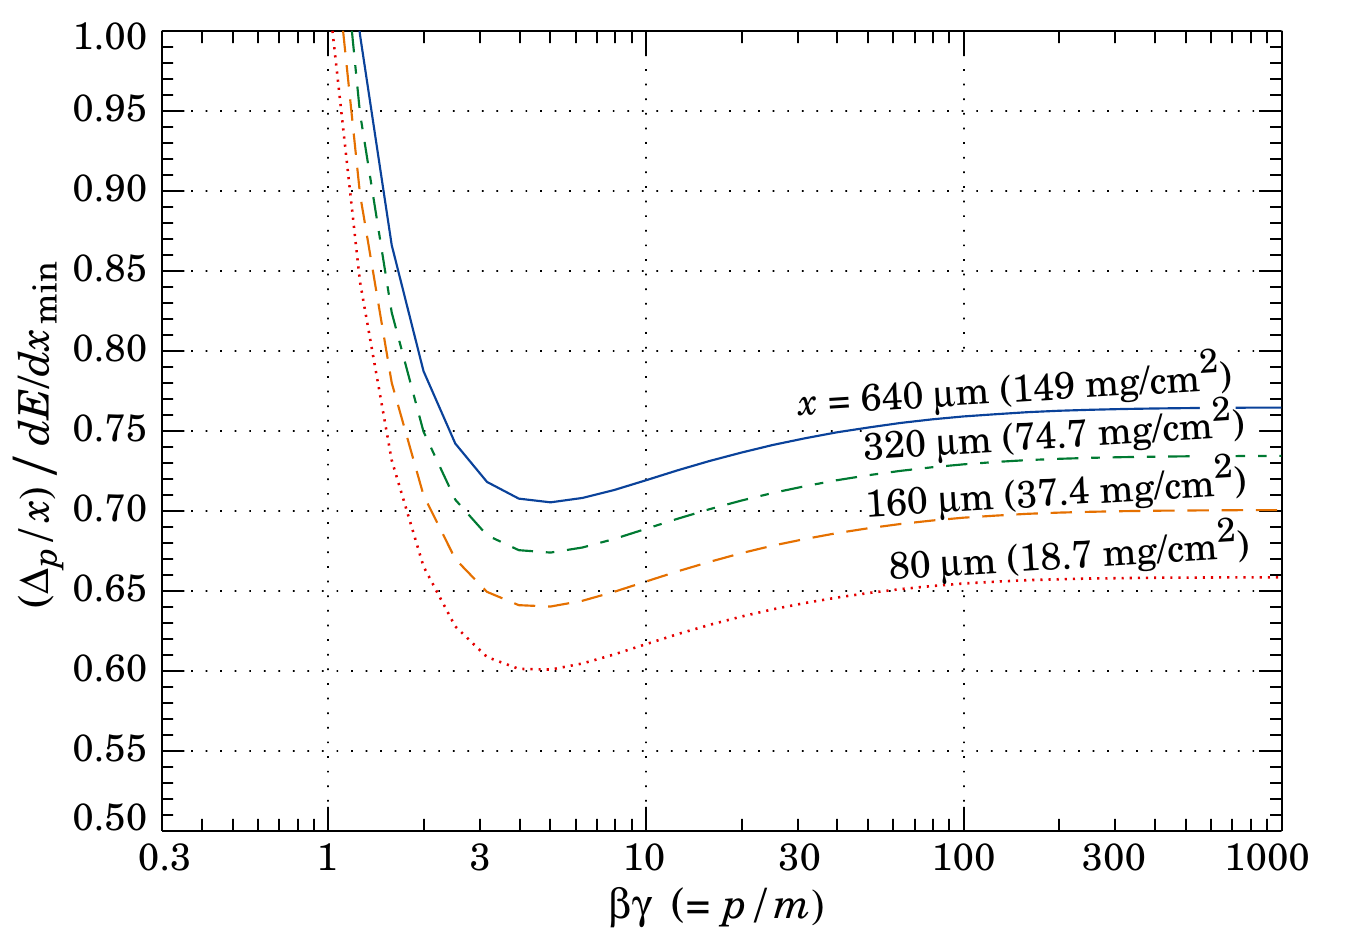
\includegraphics[width=0.6\textwidth]{figures/analysis/dEdx_Landau_Silicon.png}
  \end{tabular}
  \caption{Most probable energy loss in silicon, scaled to the mean loss of a minimal ionizing particle (388 eV/$\mu$m). Taken from \cite{bib:PDG_2014}.} 
  \label{fig:dEdx_Landau_Silicon}
\end{figure}
Thus, the energy loss per path length can be used to discriminate between SM particles and new heavy charged particles, which are usually unrelativistic because of their high mass.
%\begin{itemize}
%\item The variable dE/dx: General introdution
%\item Bethe-Bloch (difficult concept because of undefined mean of the Landau function)
%\item Landau distribution (no mean)
%\item Most probable energy loss landau vavilov function (show comparison plot Landau, Bethe)
%\item Minimal ionising particles (pt cut) (how dedx for pions CMS 2008)
%\end{itemize}

\subsection{Gain calibration of the silicon pixel tracker}

During Run I in 2012, the pixel silicon detector was continously subjected to an energy calibration, a so-called gain calibration.
Every pixel was calibrated to the same response, such that the whole pixel tracker should have been well inter-calibrated.
Unfortunately, due to various reasons, such as the imperfect constancy of the reference signal, or radiation and temperature induced changes, the energy calibration could not ensure a fully calibrated pixel tracker.
%was not adequate enough to use the measured energy deposition without a further offline calibration procedure.
This imperfection of the gain calibration can be seen in Fig.~\ref{fig:StabilityPlot_beforeCalibration}, where the sum of the harmonic-2 estimator for all tracks $\sum\limits_{\text{all trks}}I_{h2}$ over the full data-taking period in 2012 is shown.
Four different steps can be spotted.
\begin{figure}[!b]
  \centering 
  \begin{tabular}{c}
  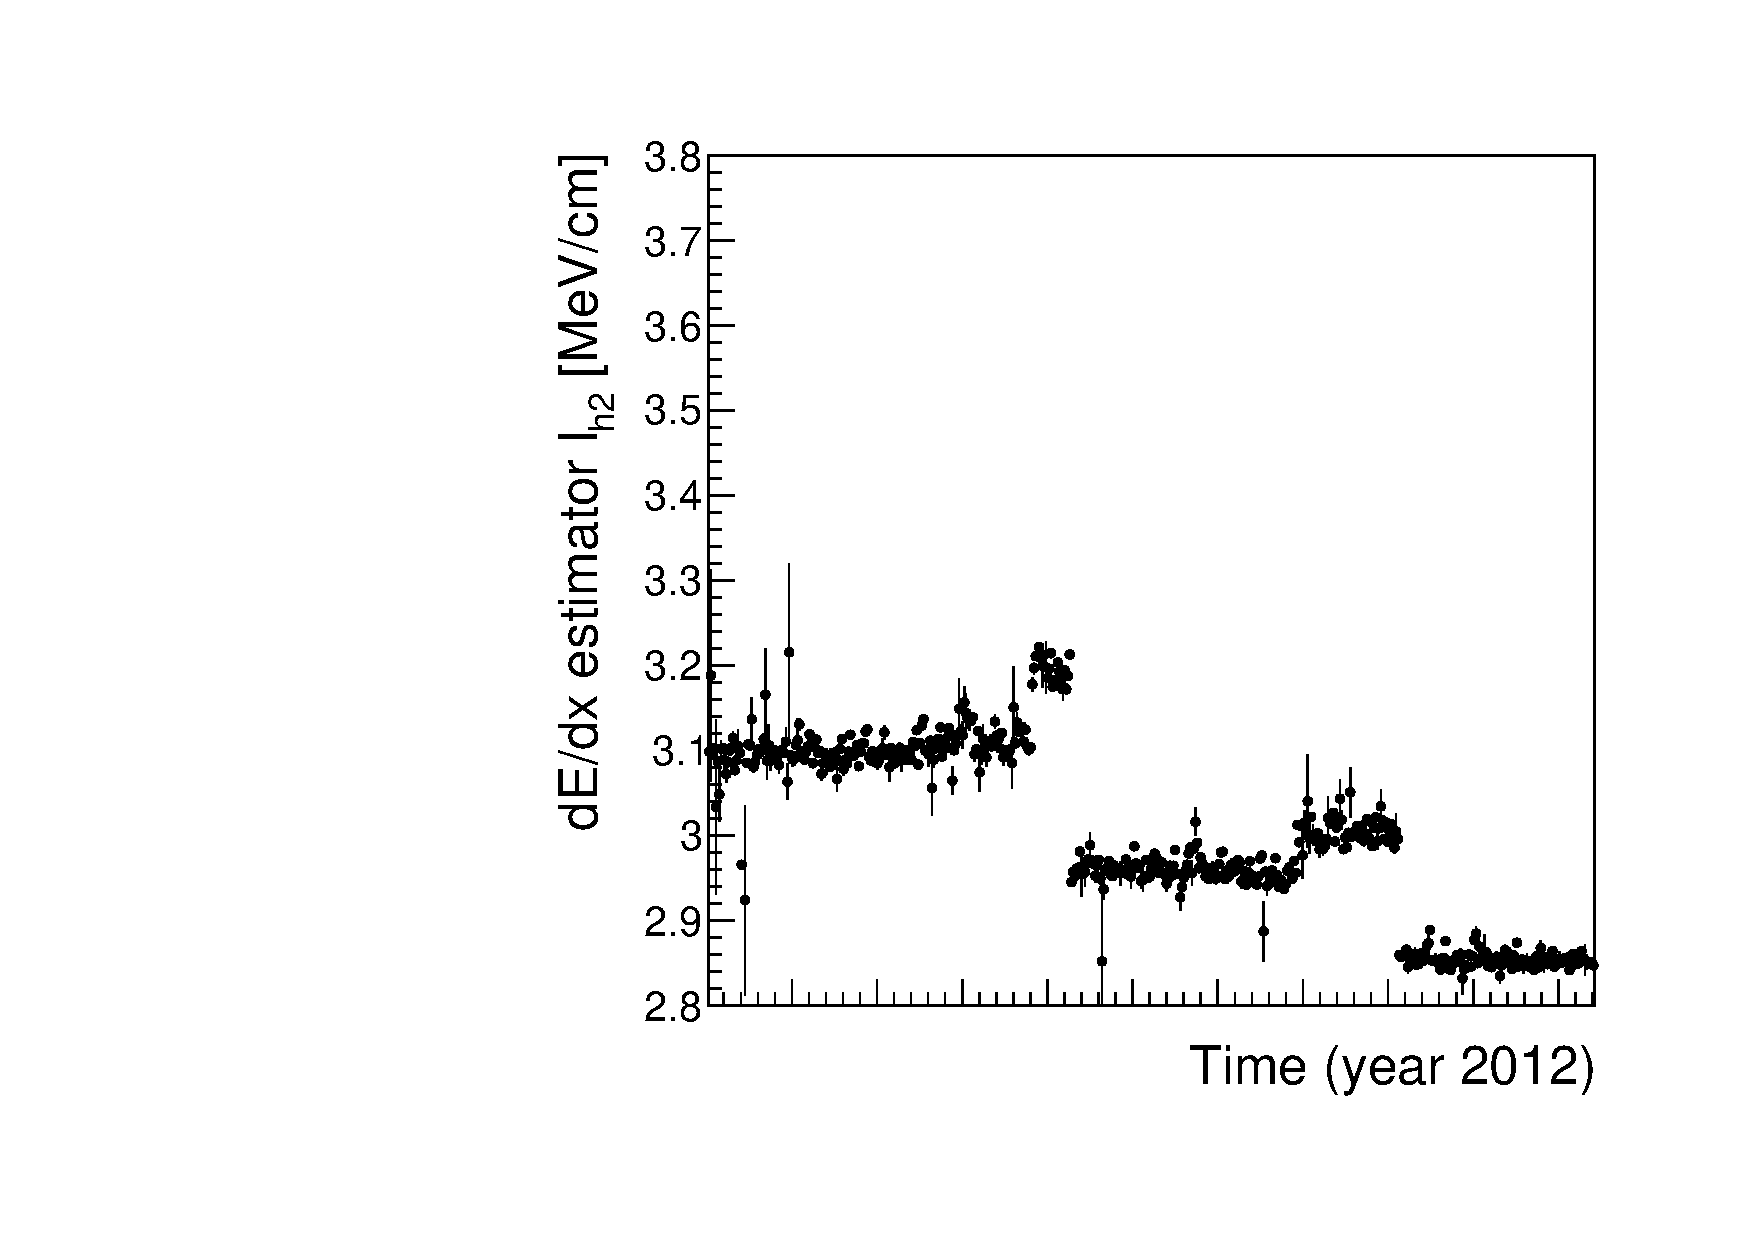
\includegraphics[width=0.49\textwidth]{figures/analysis/StabilityPlot_Pixel_beforeCalibration_withoutStepFits_NEW.pdf}
  \end{tabular}
  \caption{Sum of all track's $dE/dx$ (harmonic-2 estimator) over the full year 2012. Only pixel hits are taken into account. Every data point corresponds to one run.} 
  \label{fig:StabilityPlot_beforeCalibration}
\end{figure}
The first and the third steps correspond to changes in the settings of the tracker due to irradiation.
The second and fourth step show the moment where an online gain calibration was again applied.
Unfortunately, although a gain calibration was carried out (even with some delay), it could not bring the average dE/dx to the same level before the changes in the settings occured.
The size of the difference in the dE/dx measurement over time being around 15\% is too large to use dE/dx without a further calibration.

In the following sections the method of the gain calibration (splitted into an section about the inter-calibration of gain and the absolute calibration of gain) of the pixel silicon tracker is explained. 
Detailed technical information about the pixel tracker can be found in Sec.~\ref{sec:Detector:Pixel}.


\subsubsection*{Inter-calibration of gain}
The main goal of the gain calibration is to get a uniform response in the ionization energy loss $dE/dx$ over the full data taking period in 2012.
To ensure also a uniform response of all modules within one time step, also an inter-calibration on module level was carried out.
The inter-calibration can in principle be done on various stages: the highest granularity would be a calibration on pixel level, followed by a calibration on ROC-level and then on module-level.
Lower granularities in descending order are rings (modules with same z-position) and finally layers (3 layers in the barrel and 4 disks in the endcap). 
It was checked that all pixels and all ROCs (on one module) are well inter-calibrated, such that the inter-calibration was finally done module-wise.
%Of course, as a final step the well inter-calibrated pixel tracker within space and time, needs to be calibrated to the correct energy release of a MIP, to have a meaningful physical quantity.
%Therefore, as a last step an overall calibration factor $c_{\text{strip}}$ was determined to calibrate the average energy deposition (using the harmonic-2 estimator) of all tracks in the pixel tracker to the average energy release in the silicon strip detector.
%This can be done because the strip tracker has already been calibrated in Run I within the following analysis \cite{bib:CMS:HSCP_8TeV}.
The applied method for the gain calibration of the pixel tracker follows closely the method in \cite{bib:Quertenmont_2010}.

The gain calibration of the pixel silicon tracker has been carried out with the help of minimal ionising particles (MIPs).
MIPs in this context are not defined as particles depositing a minimum amount of energy, but more generally a small amount of energy.
This denotes all particles located at the plateau of the $dE/dx$ distribution vs. momentum (see Fig.~\ref{fig:dEdx_Landau_Silicon}).
It ensures that all particles deposit a rather similar amount of energy such that the variation due to different momenta is suppressed.
The small ionisation for particles was ensured with a momentum selection of $\text{p}>2\,$\gev.
For the calibration a sample containg around $~$50 million ``minimum bias'' events is used which is specifically recorded for tracker calibration purposes.
``Minimum bias`` means that neither an online nor offline selection was applied.

For every module in the pixel tracker (there are 1440 modules in total), a distribution of the energy loss per path length $\Delta E/\Delta x$ is built.
%each $\Delta E/\Delta x$  measurement of all particles crossing the module is filled into a histogram. 
Fig.~\ref{fig:dEdx_Module} shows an example distribution for one module.
\begin{figure}[!bt]
  \centering 
  \begin{tabular}{c}
  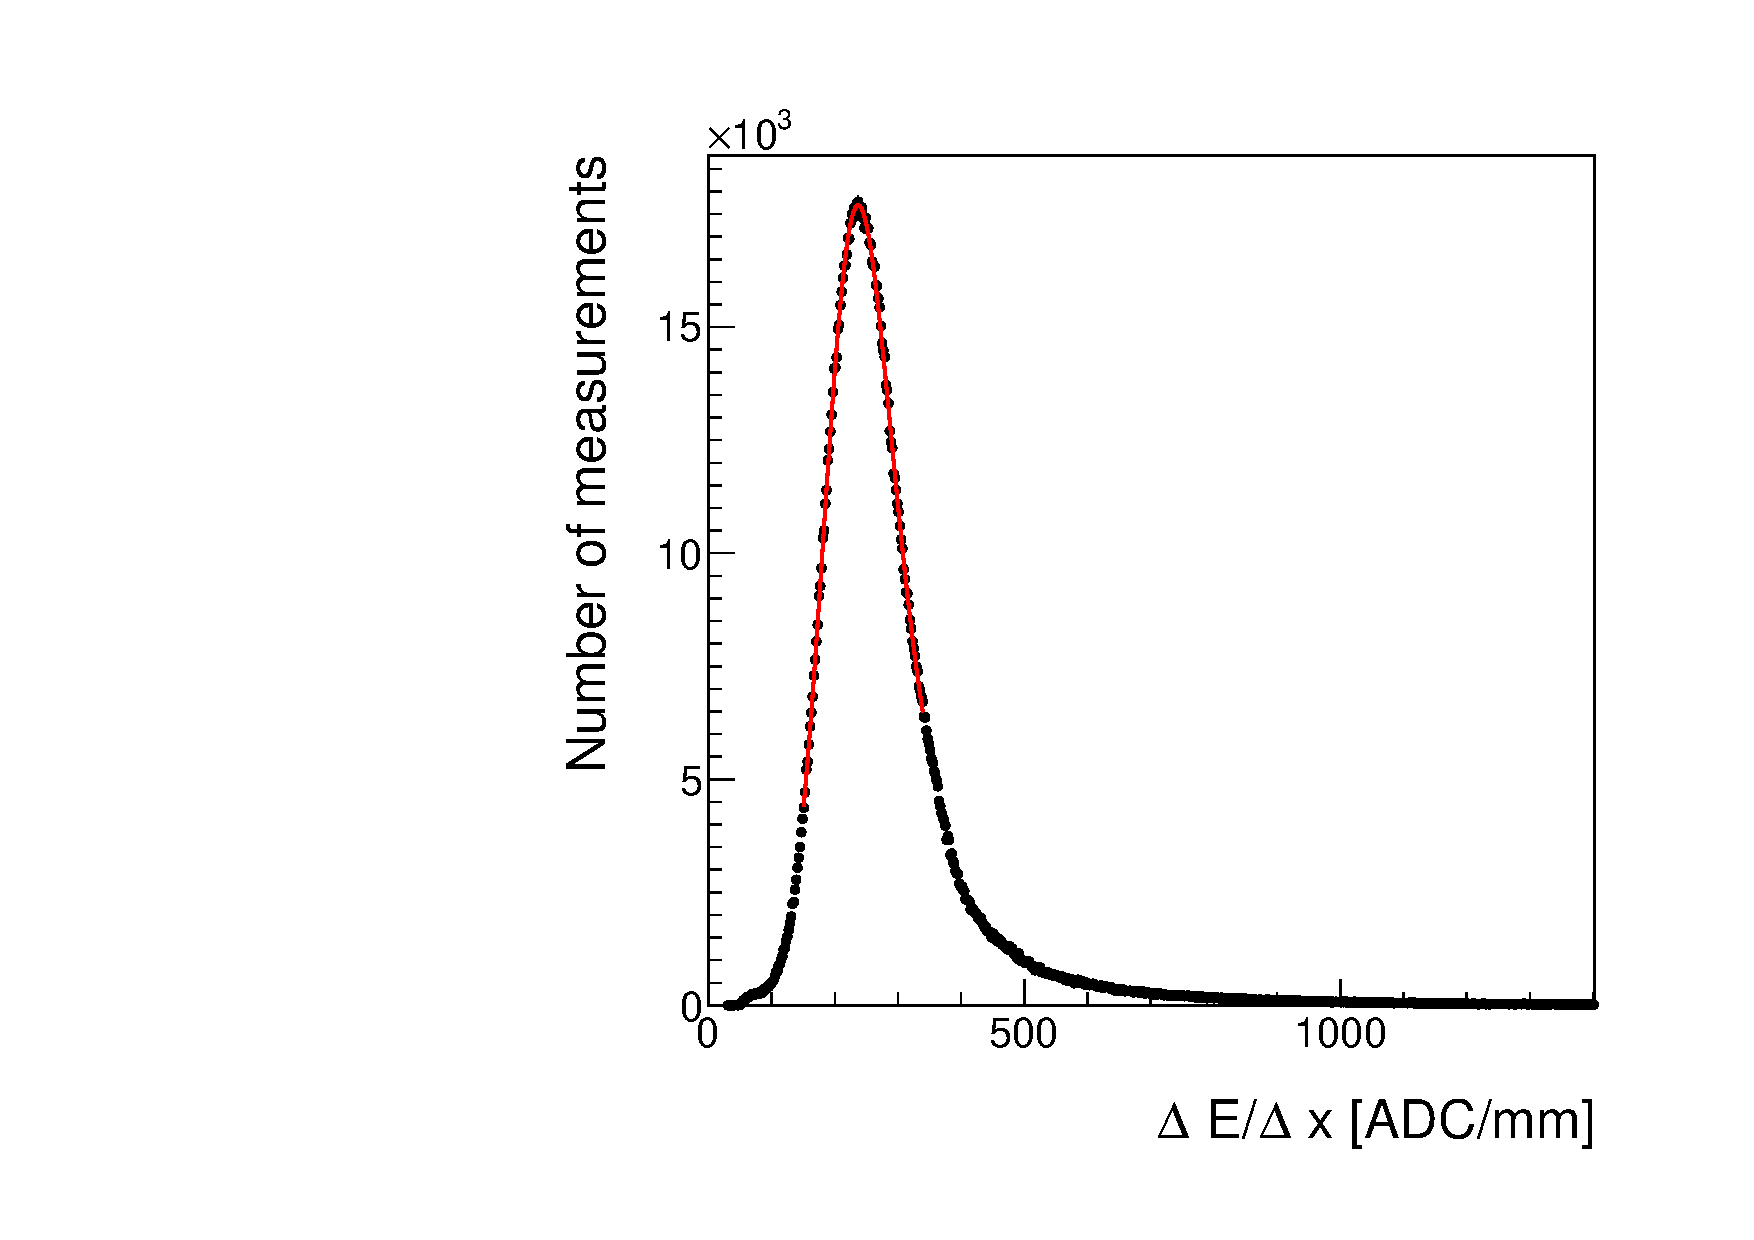
\includegraphics[width=0.49\textwidth]{figures/analysis/Landau_Module_352476680.pdf}
  \end{tabular}
  \caption{An example of the $\Delta E/\Delta x$ distribution measured in ADC count per mm for one module of the CMS pixel tracker. 
           A Landau convoluted with a Gaussian is fitted to the core of the distribution in an iterative procedure.} 
  \label{fig:dEdx_Module}
\end{figure}
The underlying Landau distribution can be nicely seen. 
To extract the MPV for every module a fit to the core distribution is performed.
The fit is done with a Landau convoluted with a Gaussian function to be closer to the experimentally observed energy spectrum.
This also increases the fit performance and the stability of the fit.
The measurement of $\Delta E/\Delta x$ is done in ADC counts per mm.
ADC counts are a measure for the deposited charge after digitization.
It consists out of a unsigned 16-bit integer (ranging from 0 to 65\,535).
The path length $\Delta x$ is calculated with
\begin{equation*}
\Delta x = d_{\text{module}_i} \cdot \cos(\phi_{\text{track}}),
\end{equation*}
where $d_{\text{module}_i}$ is the thickness of module i and $\phi_{\text{track}}$ is the relative angle of the particle's trajectory to the axis normal of the module.
With the measured MPV extracted from the fit, an inter-calibration factor is calculated for every module
\begin{equation*}
c_{\text{inter}}=\frac{\mpv\, [\text{ADC/mm}]}{\mpv_{\text{target}}\, [\text{ADC/mm}]} = \frac{\mpv\, [\text{ADC/mm}]}{300 \cdot 265 \, \text{ADC/mm}}.
\end{equation*}
The factor 300 $\cdot$ 265 ADC/mm is in principal an abitrary number. 
However, it was choosen such that it corresponds approximately to the most probably energy deposition of a MIP.
The calibration factor can then be used to scale every single measurement in a module to a calibrated $\Delta E/\Delta x$ measurement
\begin{equation*}
\frac{\Delta E}{\Delta x}_{\text{calibrated}}=\frac{\frac{\Delta E}{\Delta x}_{\text{uncalibrated}}}{c_{\text{inter}}}
\end{equation*}
The determination of the calibration factor needs to be done for every of the five time steps, shown in Fig.~\ref{fig:StabilityPlot_beforeCalibration} independently, in order to get rid of the time dependency. 
The result of the inter-calibration can be seen in Fig.~\ref{fig:StabilityPlot_afterCalibration}.
The variation over time was indeed eridicated, resulting in a maximal time variation of less than $\sim1$\%.
\begin{figure}[!bt]
  \centering 
  \begin{tabular}{c}
  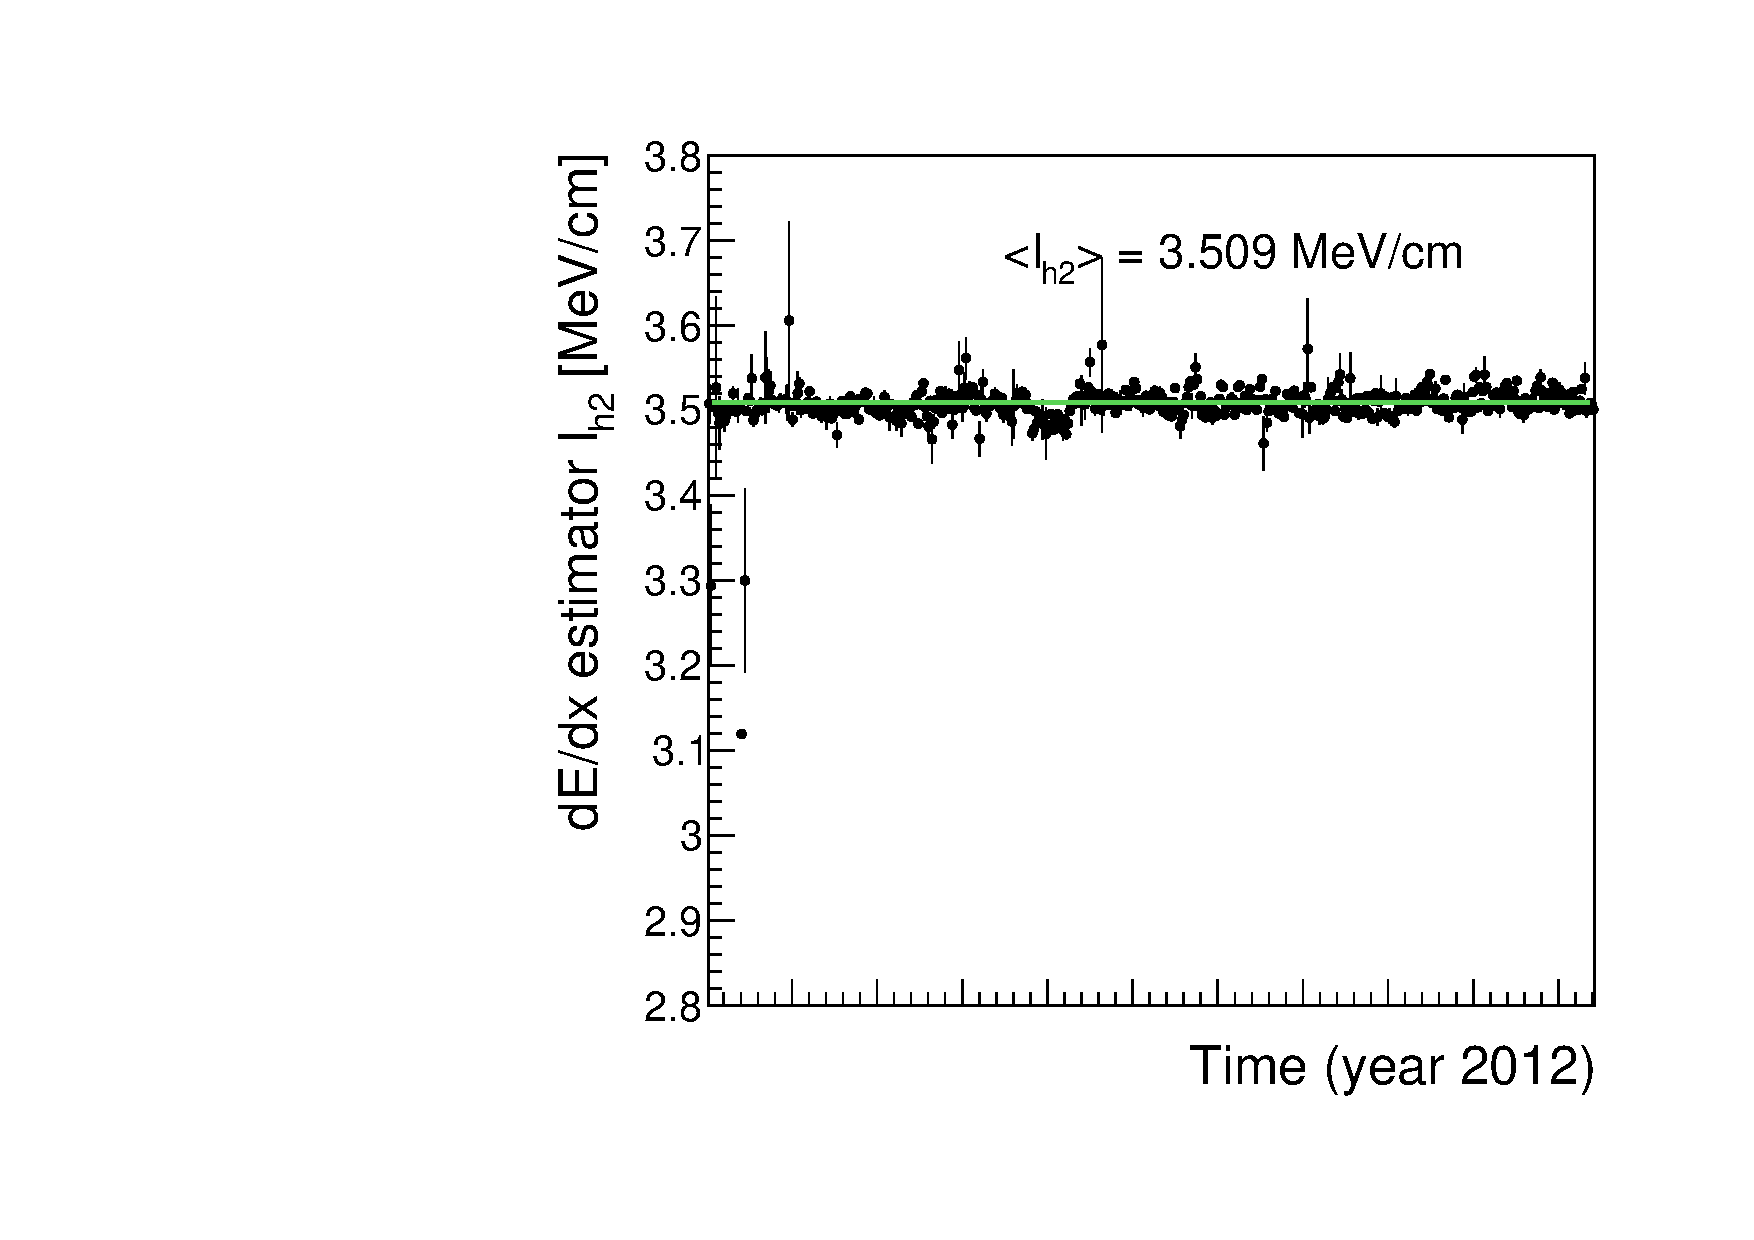
\includegraphics[width=0.49\textwidth]{figures/analysis/StabilityPlot_Pixel_afterCalibration_withoutStepFits_NEW.pdf}
  \end{tabular}
  \caption{Sum of all track's $dE/dx$ (harmonic-2 estimator) over the full year 2012 after applying the calibration factors, resulting in an average $dE/dx$ of 3.51 MeV/cm. Only pixel hits are taken into account. Every data point corresponds to one run.} 
  \label{fig:StabilityPlot_afterCalibration}
\end{figure}

Additionaly, the same procedure is carried out for a corresponding simulated data sample to ensure also the inter-calibration of the pixel modules on all simulated samples.




\subsubsection*{Absolute calibration of gain}
As a final step, the targeted \mpv being $\mpv_{\text{target}}=300 \cdot 265 \,  \text{ADC/mm}$ needs to be translated to a meaningful physical quantity given in phsical units (e.g. MeV/cm).
That means, that the charge measurement in ADC counts needs to be converted to the real energy release of a particle.
The relation between $\Delta E$ in ADC counts and the energy loss in eV is given by
\begin{equation*}
\Delta E\,[\ev] = \frac{\Delta E\,[\text{ADC}]}{c_{\text{inter}}} \cdot \frac{N_e}{\text{ADC}} \cdot 3.61 \, \ev,
\end{equation*}
where $N_e$/ADC is the number of electrons which correspond to one ADC count and 3.61\,\ev is the  mean energy needed to create one electron-hole pair in silicon at -10$\degree$C.
Such an absolute gain calibration can be done with the help of several methods (all explained in \cite{bib:Quertenmont_2010}).
For the absolute calibration of the silicon pixel tracker, it can be taken advantage of the already conducted absolute calibration of the silicon strip detector.
In \cite{bib:Quertenmont_2010}, the absolute gain calibration was done with the help of the most probable energy release per path length of muons, 
theoretically described by the Landau-Vavilov-Bichsel formula in Eq.~\ref{eq:Landau_Vavilov_Bichsel}.  
To calibrate the pixel tracker to the correct energy loss per path length it is therefore sufficient to determine one calibration factor to relate the average $dE/dx$ of all tracks in the pixel tracker as shown in 
Fig.~\ref{fig:StabilityPlot_afterCalibration} to the average measured $dE/dx$ in the strip tracker, shown in Fig.~\ref{fig:StabilityPlot_Strip} by
\begin{equation*}
c_{\text{absolute}} = \frac{dE/dx_{\text{strip}}}{dE/dx_{\text{pixel}}} = \frac{3.303}{3.509} = 0.941.
\end{equation*}
\begin{figure}[!bt]
  \centering 
  \begin{tabular}{c}
  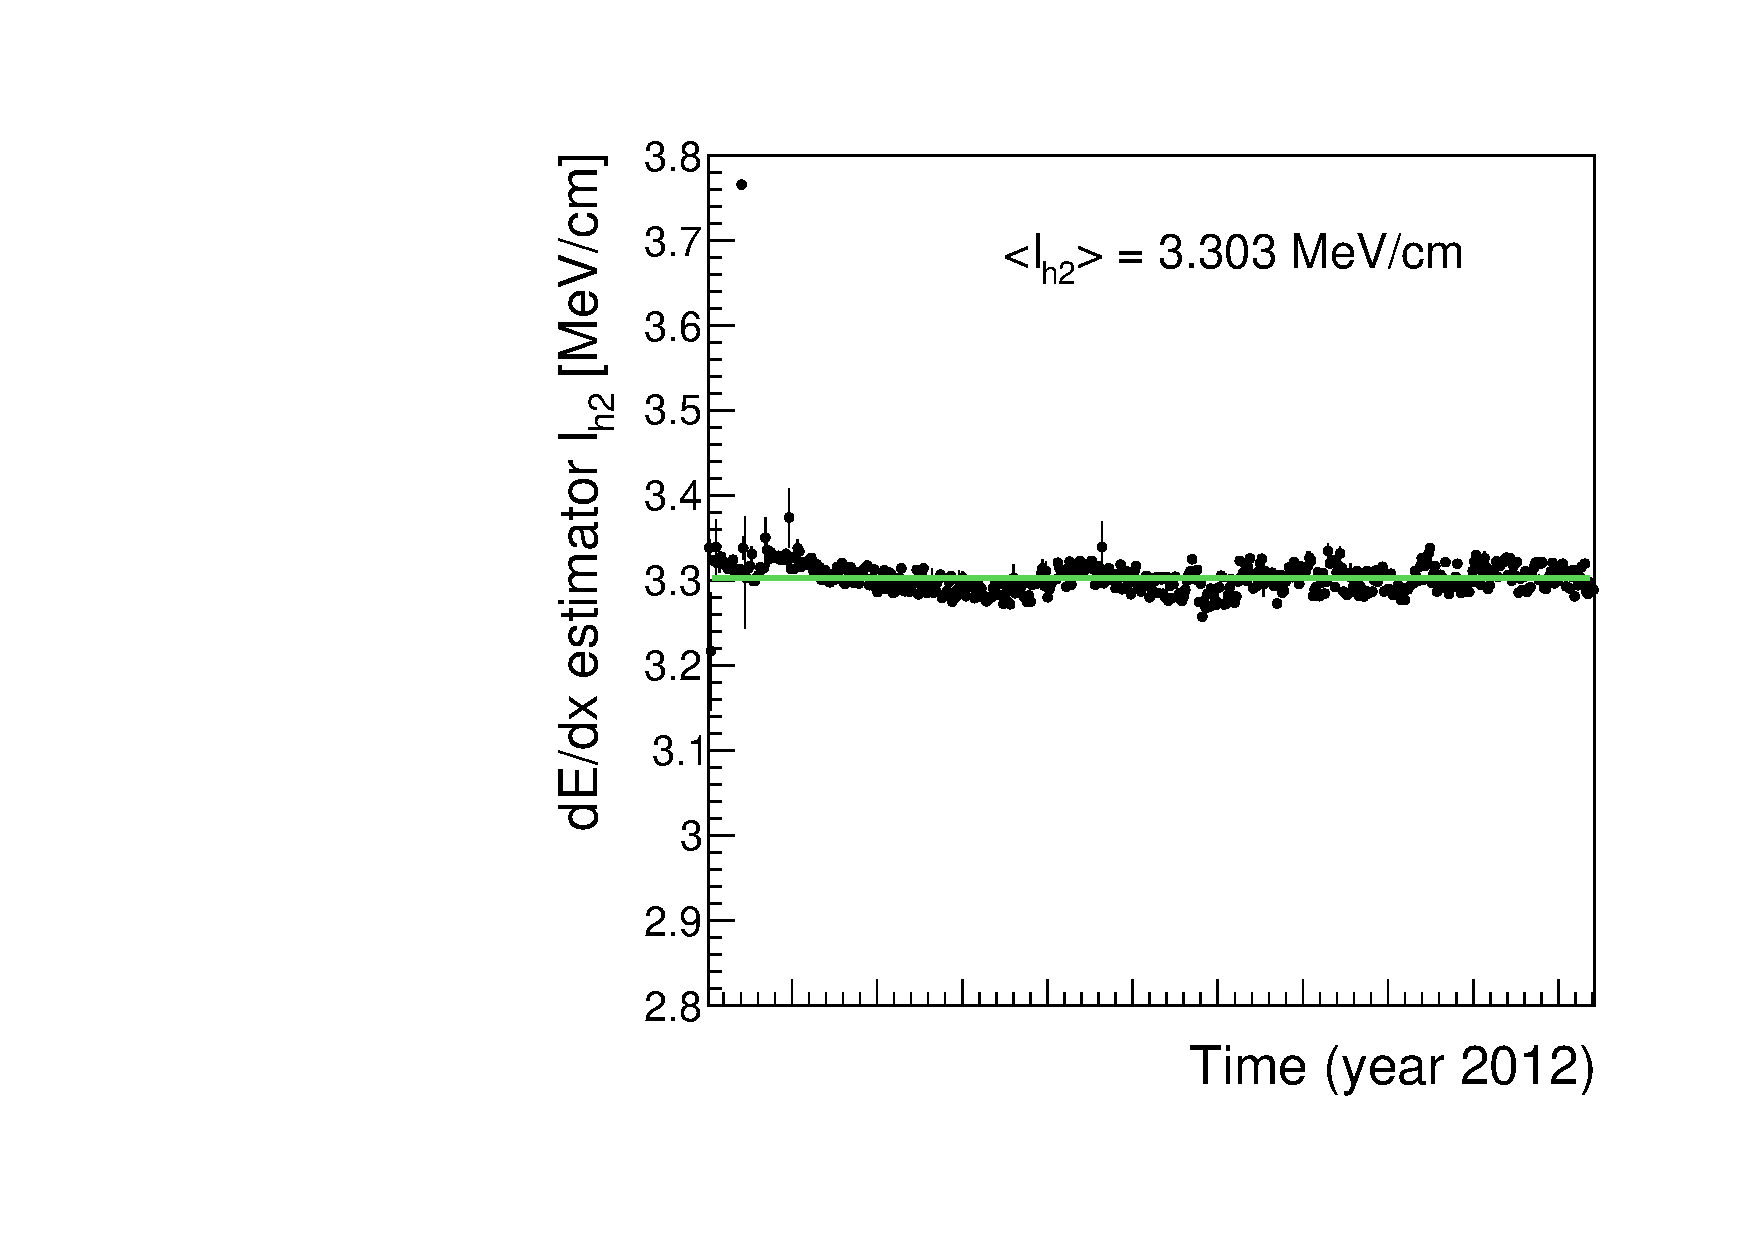
\includegraphics[width=0.49\textwidth]{figures/analysis/StabilityPlot_Strip_afterCalibration_withoutStepFits_NEW.pdf}
  \end{tabular}
  \caption{Sum of all track's $dE/dx$ (harmonic-2 estimator) measured in the silicon strip detector over the full year 2012. The average most probable $dE/dx$ is $I_{h2}=3.303\,\mev/\cm$. Every data point corresponds to one run.} 
  \label{fig:StabilityPlot_Strip}
\end{figure}
This factor is then applied on top of $c_{\text{inter}}$ for all pixel modules.

Finally, also for the simulated samples an absolute calibration factor needs to be determined, where the simulated pixel tracker is  calibrated to the average $dE/dx$ of the silicon strip measured in data.

\subsection{Asymmetric Smirnov discriminator}

As mentioned before, a difficult task when measuring the energy deposition of a particle consists in finding a robust estimator for the MPV of the underlying Landau, i.e combining eventually only a few single measurements of $\Delta E/ \Delta x$ to one single $dE/dx$ estimator.
The harmonic-2 estimator $I_{h2}$ was already introduced in Sec.~\ref{sec:sub:MeasuringDeDx} in Eq.~\ref{eq:Harmonic2Estimator}.
It is known as a robust estimator not easily biased by large fluctuation in $\Delta E/ \Delta x$ because of the suppression by a factor of 2.

However, it was shown in \cite{bib:Quertenmont_2010} that a better discrimination between SM particles and possible new heavy particles can be achieved when using likelihood techniques,
i.e. determining the probability that the set of all $\Delta E/ \Delta x$ belonging to one track is actually compatible with the hypothetical probability distribution of a MIP.

Testing that a measured sample has been drawn from a specific distribution is know as the Smirnov-Cram\'{e}r-von Mises test \cite{bib:Anderson:CramerVonMises_1962,bib:James:StaticticalMethods_2006},
which is deduced from the integral of the squared difference of the measured distribution $P_N(x)$ to the hypothesis distribution $P(x)$
\begin{equation*}
I_s = \int\limits_{-\infty}^{\infty} \left[P_{N}(x)-P(x)\right]^2 dP(x)
\end{equation*}
leading to a test statistics of
\begin{equation*}
I_s = \frac{3}{N} \cdot \left( \frac{1}{12N} + \sum\limits_{i=1}^N \left[ P_i - \frac{2i-1}{2N} \right]^2 \right),
\end{equation*}
where $P_i$ is the cumulative probability that a MIP would release a $\Delta E/\Delta x$ equal or smaller than the measured $\Delta E/ \Delta x$ with all $P_i$ are arranged in increasing order.

However, this test statistics is not sensitive to whether there are incompatibilities because of higher or lower variations compared to the hypothesis distribution.
It is therefore not really suitable for the discrimination between MIPs and heavy new particles by $dE/dx$.
A so-called Asymmetric Smirnov-Cram\'{e}r-von Mises discriminator was developed in \cite{bib:Quertenmont_2010} which is only sensitive to incompatibilites to the MIP hypothesis towards higher energy depositions
\begin{equation*}
I_{as} = \frac{3}{N} \cdot \left( \frac{1}{12N} + \sum\limits_{i=1}^N \left[ P_i \cdot \left(P_i - \frac{2i-1}{2N} \right)^2 \right] \right).
\end{equation*}
A value of $I_{as}$ close to zero indicates good compatibility with the MIP hypothesis, whereas a value close to one indicates worse compatibility because of too large energy loss.

The underlying probability distribution of the energy release for a given path length in the pixel tracker is extracted from the same ``Minimum bias'' sample used for the pixel energy calibration.
In total 28 different templates each for a different given path length are created.
The corresponding templates for the energy release in the silicon strip detector were already built by  \cite{bib:Quertenmont_2010}.
In Fig.~\ref{fig:ProbabilityTemplate} the probability distribution template for the pixel tracker in data and simulation is shown.
\begin{figure}[!tb]
  \centering 
  \begin{tabular}{c}
    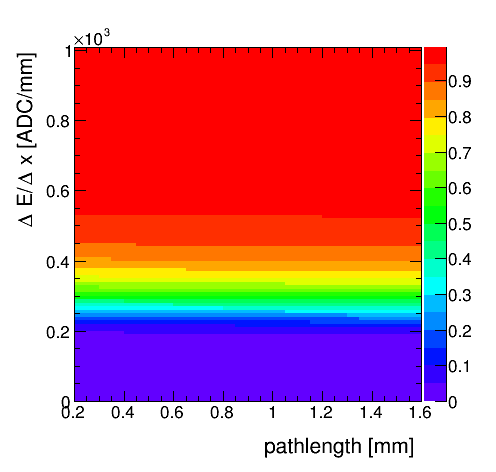
\includegraphics[width=0.49\textwidth]{figures/analysis/Discriminator_template_data_pixel_2012.png}
    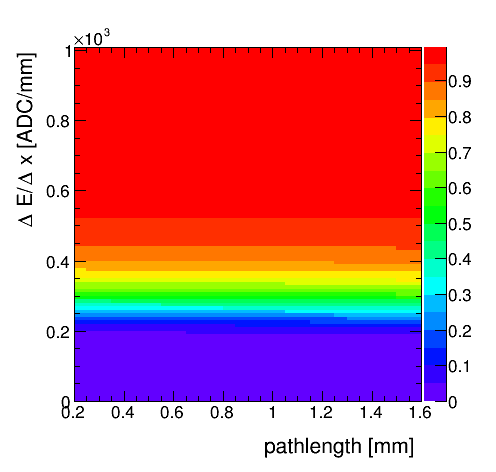
\includegraphics[width=0.49\textwidth]{figures/analysis/Discriminator_template_mc_pixel_2012.png}
  \end{tabular}
  \caption{Cumulative probability for a MIP to release a $\Delta E/ \Delta x$ (y-axis) vs. the pathlength (x-axis) in data (left) and simulation (right) for the pixel tracker.}
  \label{fig:ProbabilityTemplate}
\end{figure}
The distribution of the Asymmetric Smirnov-Cram\'{e}r-von Mises discriminator $I_{as}$ (for simplicity $I_{as}$ will be just called Asymmetric Smirnov discriminator in the following text) can be found in Fig.~\ref{blbla}, 
where the energy release per pathlength for MIPs in  data and simulation is drawn.
It shows good agreement.\\

As already pointed out several times, the goal of including the pixel energy information is to increase the discrimination power of $I_{as}$ between background and signal, especially for short tracks.
In Fig.~\ref{}, a comparison of the shapes of background tracks and signal tracks in simulated samples without any selection is shown (details on the Simulated samples can be found in Sec.~\ref{sec:SimulatedSamples}).
It can be seen, that the $I_{as}$ distribution of the signal tracks shows a much longer tails toward the right end of the plot, whereas the background is rather distributed close to zero.
Not only the mass of the signal track influences the $I_{as}$ distribution but also the number of hits of a signal track which in turn define the influence of fluctuations of single $\Delta E/\Delta x$ measurements on the $I_{as}$ discriminator. 
This is shown in Fig.~\ref{...}.


\subsection{Efficiency improvements}
In order to quantify the impact of the additional pixel $\Delta E/\Delta x$ information on an analysis selection, the signal selection efficiency over the background selection efficiency for different selection cuts of $I_{as}$ is drawn in Fig.~\ref{blabla}.
As can be seen, the improved background supression for a given signal selection efficiency depends on the mass and on the lifetime of the chargino.
For masses of blablab, improvements in the backgorund supression of .... can be achieved.
For low lifetimes, the additionnaly improves up to a factor of ....


\begin{itemize}
\item Show comparison of Ias comparing pixel and strip
\item Show plot with Ias distribution for bkg and signal (give reference to next chapter)
\item not a long section
\end{itemize}
In Fig.~\ref{blbla}, a comparison between signal sample and background dedx is shown. It can be already seen that $I_{as}$ is well discriminating.


%%%%%%%%%%%%%%%%%%%%%%%%%%%%%%%%%%%%%%%%%%%%%%%%%%%%%%%%%%%%%%%%%%%%%%%%%%%%%%%%%%%%%%%%%%%%%%%%%%%%%%%%%%%%%%%%%%%%%%%%%%%%%%%%%%%%%%%%%%%%%%%%%%%%%%%%%%%%%%%%%%%%%%%%%%%%%%%%%%%%
%%%%%%%%%%%%%%%%%%%%%%%%%%%%%%%%%%%%%%%%%%%%%%%%%%%%%%%%%%%%%%%%%%%%%%%%%%%%%%%%%%%%%%%%%%%%%%%%%%%%%%%%%%%%%%%%%%%%%%%%%%%%%%%%%%%%%%%%%%%%%%%%%%%%%%%%%%%%%%%%%%%%%%%%%%%%%%%%%%%%
\section{Simulated samples}
\label{sec:SimulatedSamples}

\begin{itemize}
\item Event weights applied for correct Pileup modelling
\item Detailed information can be found in Experimental setup chapter
\item Think what to write in the detector chapter to be not wiederholend     
\end{itemize}

Detector chapter:
\begin{itemize}
\item THINK!
\end{itemize}

\subsection{SM samples}
\begin{itemize}
\item Title: Background samples
\item To study the background, following samples were used: ... generated with ...
\item Not all SM processes samples were availbale
\item Not so dramatic, because data based bkg estimation method
\item Main Background are ... ???
\item Only a few were available and thus processed
\item Most important sample was included: Wjets
\item ZoNuNu Backgorund not availbale plays also a role (see DT paper!)
\item Table of SM samples with cross-sections
\end{itemize}

\subsection{Signal samples}
\begin{itemize}
\item Lifetime reweighting
\item Simulation of lifetime in Geant
\item Trigger emulation
\item What samples are exactly generated.
\item Madgraph+Pythia
\item Chargino Pair production + Chargino neutralino production
\item Table with generated signal samples with cross-sections???? No
\end{itemize}

%%%%%%%%%%%%%%%%%%%%%%%%%%%%%%%%%%%%%%%%%%%%%%%%%%%%%%%%%%%%%%%%%%%%%%%%%%%%%%%%%%%%%%%%%%%%%%%%%%%%%%%%%%%%%%%%%%%%%%%%%%%%%%%%%%%%%%%%%%%%%%%%%%%%%%%%%%%%%%%%%%%%%%%%%%%%%%%%%%%%
%%%%%%%%%%%%%%%%%%%%%%%%%%%%%%%%%%%%%%%%%%%%%%%%%%%%%%%%%%%%%%%%%%%%%%%%%%%%%%%%%%%%%%%%%%%%%%%%%%%%%%%%%%%%%%%%%%%%%%%%%%%%%%%%%%%%%%%%%%%%%%%%%%%%%%%%%%%%%%%%%%%%%%%%%%%%%%%%%%%%
\section{Event selection}
\label{sec:EventSelection}
\subsection{Datasets and triggers}
\begin{itemize}
\item Datasets and triggers used in the analysis
\item signal samples generated with Madgraph and pythia
\item They are decayed in Geant to only pions. Around ten different lifetimes were simulated
\item For other lifetimes: lifetime reweighting is done PLOT
\item For five diffenrent masses (100-500 GeV) 
\end{itemize}
\subsection{Preselection}
\begin{itemize}
\item Motivate different selection cuts
\item Reference DT search for most of them
\end{itemize}
\subsection{Main discriminating variables}
\begin{itemize}
\item dE/dx
\item pt
\item Show some MC signal bkg comparioson plots (only Wjets?)
\end{itemize}

%%%%%%%%%%%%%%%%%%%%%%%%%%%%%%%%%%%%%%%%%%%%%%%%%%%%%%%%%%%%%%%%%%%%%%%%%%%%%%%%%%%%%%%%%%%%%%%%%%%%%%%%%%%%%%%%%%%%%%%%%%%%%%%%%%%%%%%%%%%%%%%%%%%%%%%%%%%%%%%%%%%%%%%%%%%%%%%%%%%%
\section{Sources of backgrounds}
\label{sec:SourcesOfBackgrounds}
\begin{itemize}
\item Background consist of particles which make high energy deposits and are high pt
\item In general: Low background search
\end{itemize}
\subsection{Fake tracks}
\begin{itemize}
\item Definition of fake tracks
\item How can they fake the signal
\end{itemize}
\subsection{Muons}
\begin{itemize}
\item How can muons fake the signal
\end{itemize}
\subsection{Pions}
\begin{itemize}
\item How can pions fake the signal
\end{itemize}
\subsection{Electrons}
\begin{itemize}
\item How can electrons fake the signal
\end{itemize}
%%%%%%%%%%%%%%%%%%%%%%%%%%%%%%%%%%%%%%%%%%%%%%%%%%%%%%%%%%%%%%%%%%%%%%%%%%%%%%%%%%%%%%%%%%%%%%%%%%%%%%%%%%%%%%%%%%%%%%%%%%%%%%%%%%%%%%%%%%%%%%%%%%%%%%%%%%%%%%%%%%%%%%%%%%%%%%%%%%%%
%%%%%%%%%%%%%%%%%%%%%%%%%%%%%%%%%%%%%%%%%%%%%%%%%%%%%%%%%%%%%%%%%%%%%%%%%%%%%%%%%%%%%%%%%%%%%%%%%%%%%%%%%%%%%%%%%%%%%%%%%%%%%%%%%%%%%%%%%%%%%%%%%%%%%%%%%%%%%%%%%%%%%%%%%%%%%%%%%%%%
\section{Background estimation methods}
\label{sec:BackgroundEstimation}
\subsection{Fake background}
\subsection{Leptonic background}
\subsection{Systematic uncertainties}

%%%%%%%%%%%%%%%%%%%%%%%%%%%%%%%%%%%%%%%%%%%%%%%%%%%%%%%%%%%%%%%%%%%%%%%%%%%%%%%%%%%%%%%%%%%%%%%%%%%%%%%%%%%%%%%%%%%%%%%%%%%%%%%%%%%%%%%%%%%%%%%%%%%%%%%%%%%%%%%%%%%%%%%%%%%%%%%%%%%%
\section{Optimization of search sensitivity}
\label{sec:Optimization}
\begin{itemize}
\item Show plots
\item show table
\item Include NlostOuter here, too
\end{itemize}

%%%%%%%%%%%%%%%%%%%%%%%%%%%%%%%%%%%%%%%%%%%%%%%%%%%%%%%%%%%%%%%%%%%%%%%%%%%%%%%%%%%%%%%%%%%%%%%%%%%%%%%%%%%%%%%%%%%%%%%%%%%%%%%%%%%%%%%%%%%%%%%%%%%%%%%%%%%%%%%%%%%%%%%%%%%%%%%%%%%%
\section{Statistical Methods/ Limit setting}
\label{sec:LimitSetting}

%%%%%%%%%%%%%%%%%%%%%%%%%%%%%%%%%%%%%%%%%%%%%%%%%%%%%%%%%%%%%%%%%%%%%%%%%%%%%%%%%%%%%%%%%%%%%%%%%%%%%%%%%%%%%%%%%%%%%%%%%%%%%%%%%%%%%%%%%%%%%%%%%%%%%%%%%%%%%%%%%%%%%%%%%%%%%%%%%%%%
\section{Results}
\label{sec:Results}
\begin{itemize}
\item Data cutflowtable
\item Tables with results
\item One plot (4 bins: Prediction and data)
\end{itemize}

%%%%%%%%%%%%%%%%%%%%%%%%%%%%%%%%%%%%%%%%%%%%%%%%%%%%%%%%%%%%%%%%%%%%%%%%%%%%%%%%%%%%%%%%%%%%%%%%%%%%%%%%%%%%%%%%%%%%%%%%%%%%%%%%%%%%%%%%%%%%%%%%%%%%%%%%%%%%%%%%%%%%%%%%%%%%%%%%%%%%
\section{Interpretation}
\label{sec:Interpretation}
\subsection{Systematic uncertainties of simulated signal samples}
\subsection{Exclusion limits}
\begin{itemize}
\item 1-d limits
\item 2-d limits
\end{itemize}

